%!TEX program = xelatex
\documentclass[a4paper,12pt]{report}
\usepackage{indentfirst} 
%\usepackage{ctex}
\usepackage{xeCJK}
\usepackage{times}
\usepackage{graphicx,float}
\usepackage{setspace}
\usepackage{fancyhdr}
\usepackage{array}
\usepackage{fontspec,xunicode,xltxtra}
\usepackage{titlesec}
\usepackage{titletoc}
\usepackage[titletoc]{appendix}
\usepackage[top=30mm,bottom=30mm,left=20mm,right=20mm]{geometry}
\usepackage{cite}
\usepackage{listings}
\usepackage[framed,numbered,autolinebreaks,useliterate]{mcode}
\usepackage[UTF8]{ctex}

\XeTeXlinebreaklocale "zh"
\XeTeXlinebreakskip = 0pt plus 1pt minus 0.1pt
\usepackage[
    %colorlinks = true, % 使链接为彩色而不是有边框
    linkbordercolor = white % 将链接边框颜色设置为白色，使其不可见
]{hyperref}

% 页眉页脚设置
\fancypagestyle{plain}{\pagestyle{fancy}}
\pagestyle{fancy}
\lhead{\kaishu 数据库实验报告}
\rhead{\kaishu 实验2}
\cfoot{\thepage}

% 章节标题设置
\titleformat{\chapter}{\centering\zihao{-1}\heiti}{实验\chinese{chapter}}{1em}{}
\titlespacing{\chapter}{0pt}{*0}{*6}

% 代码样式配置
\lstset{
    language=SQL,
    basicstyle=\ttfamily\small\CJKfamily{simsun},
    commentstyle=\color{green!50!black},
    keywordstyle=\color{blue},
    stringstyle=\color{red},
    showstringspaces=false,
    breaklines=true,
    frame=single,
    numbers=left,
    numberstyle=\tiny\color{gray},
    escapeinside=``,
    literate={。}{{。}}1
            {，}{{，}}1
}

\setCJKfamilyfont{SimHei}{SimHei}[
    BoldFont = SimHei Bold,
    ItalicFont = SimHei Italic,
    BoldItalicFont = SimHei BoldItalic
]
\setCJKfamilyfont{kai}{KaiTi}
\setlength{\headheight}{14.49998pt}

% 定义封面宏
\newcommand{\makeExperimentCover}[7]{
    \begin{titlepage}
        \begin{center}
            
\includegraphics[width=1.0\textwidth]{../figure/nankai.jpg}\\
            \vspace{50mm}
            \textbf{\zihao{1}\heiti{#1}}\\[1cm]
            \textbf{\zihao{2}\heiti{(2024\textasciitilde2025学年第二学期)}}\\[1cm]
            \vspace{\fill}
            
            \setlength{\extrarowheight}{2mm}
            {\songti\zihao{3}	
            \begin{tabular}{rl}
                 实验名称：& MySQL 用户管理与复杂查询实验报告\\
                 学\qquad 院：& 软件学院\\
                 姓\qquad 名：& 郭威威\\
                 学\qquad 号：& 2414308\\
                 指导老师：& 李旭东\\
            \end{tabular}
            }\\[2cm]
            \vspace{\fill}
            \zihao{4}
            2024\textasciitilde 2025春季学期\\
            使用\LaTeX 撰写于 \today
        \end{center}	
    \end{titlepage}
}

\begin{document}
% 调用封面宏生成封面
\makeExperimentCover{MySQL数据库操作实验报告}{MySQL数据库综合操作实验}{你所在学院}{你的姓名}{你的学号}{指导老师姓名}

% 目录
\tableofcontents

% 正文内容区域
\begin{spacing}{1.5}
\songti\zihao{-4}

\chapter{实验目的}
本次实验聚焦于MySQL数据库操作，旨在熟练掌握Python与MySQL的交互、MySQL用户权限管理、数据库及表的创建与数据导入，以及复杂查询操作，提升数据库实践能力。

\chapter{实验环境}
\section{操作系统}
Windows 11 Pro 22H2

\section{软件版本}
\begin{center}
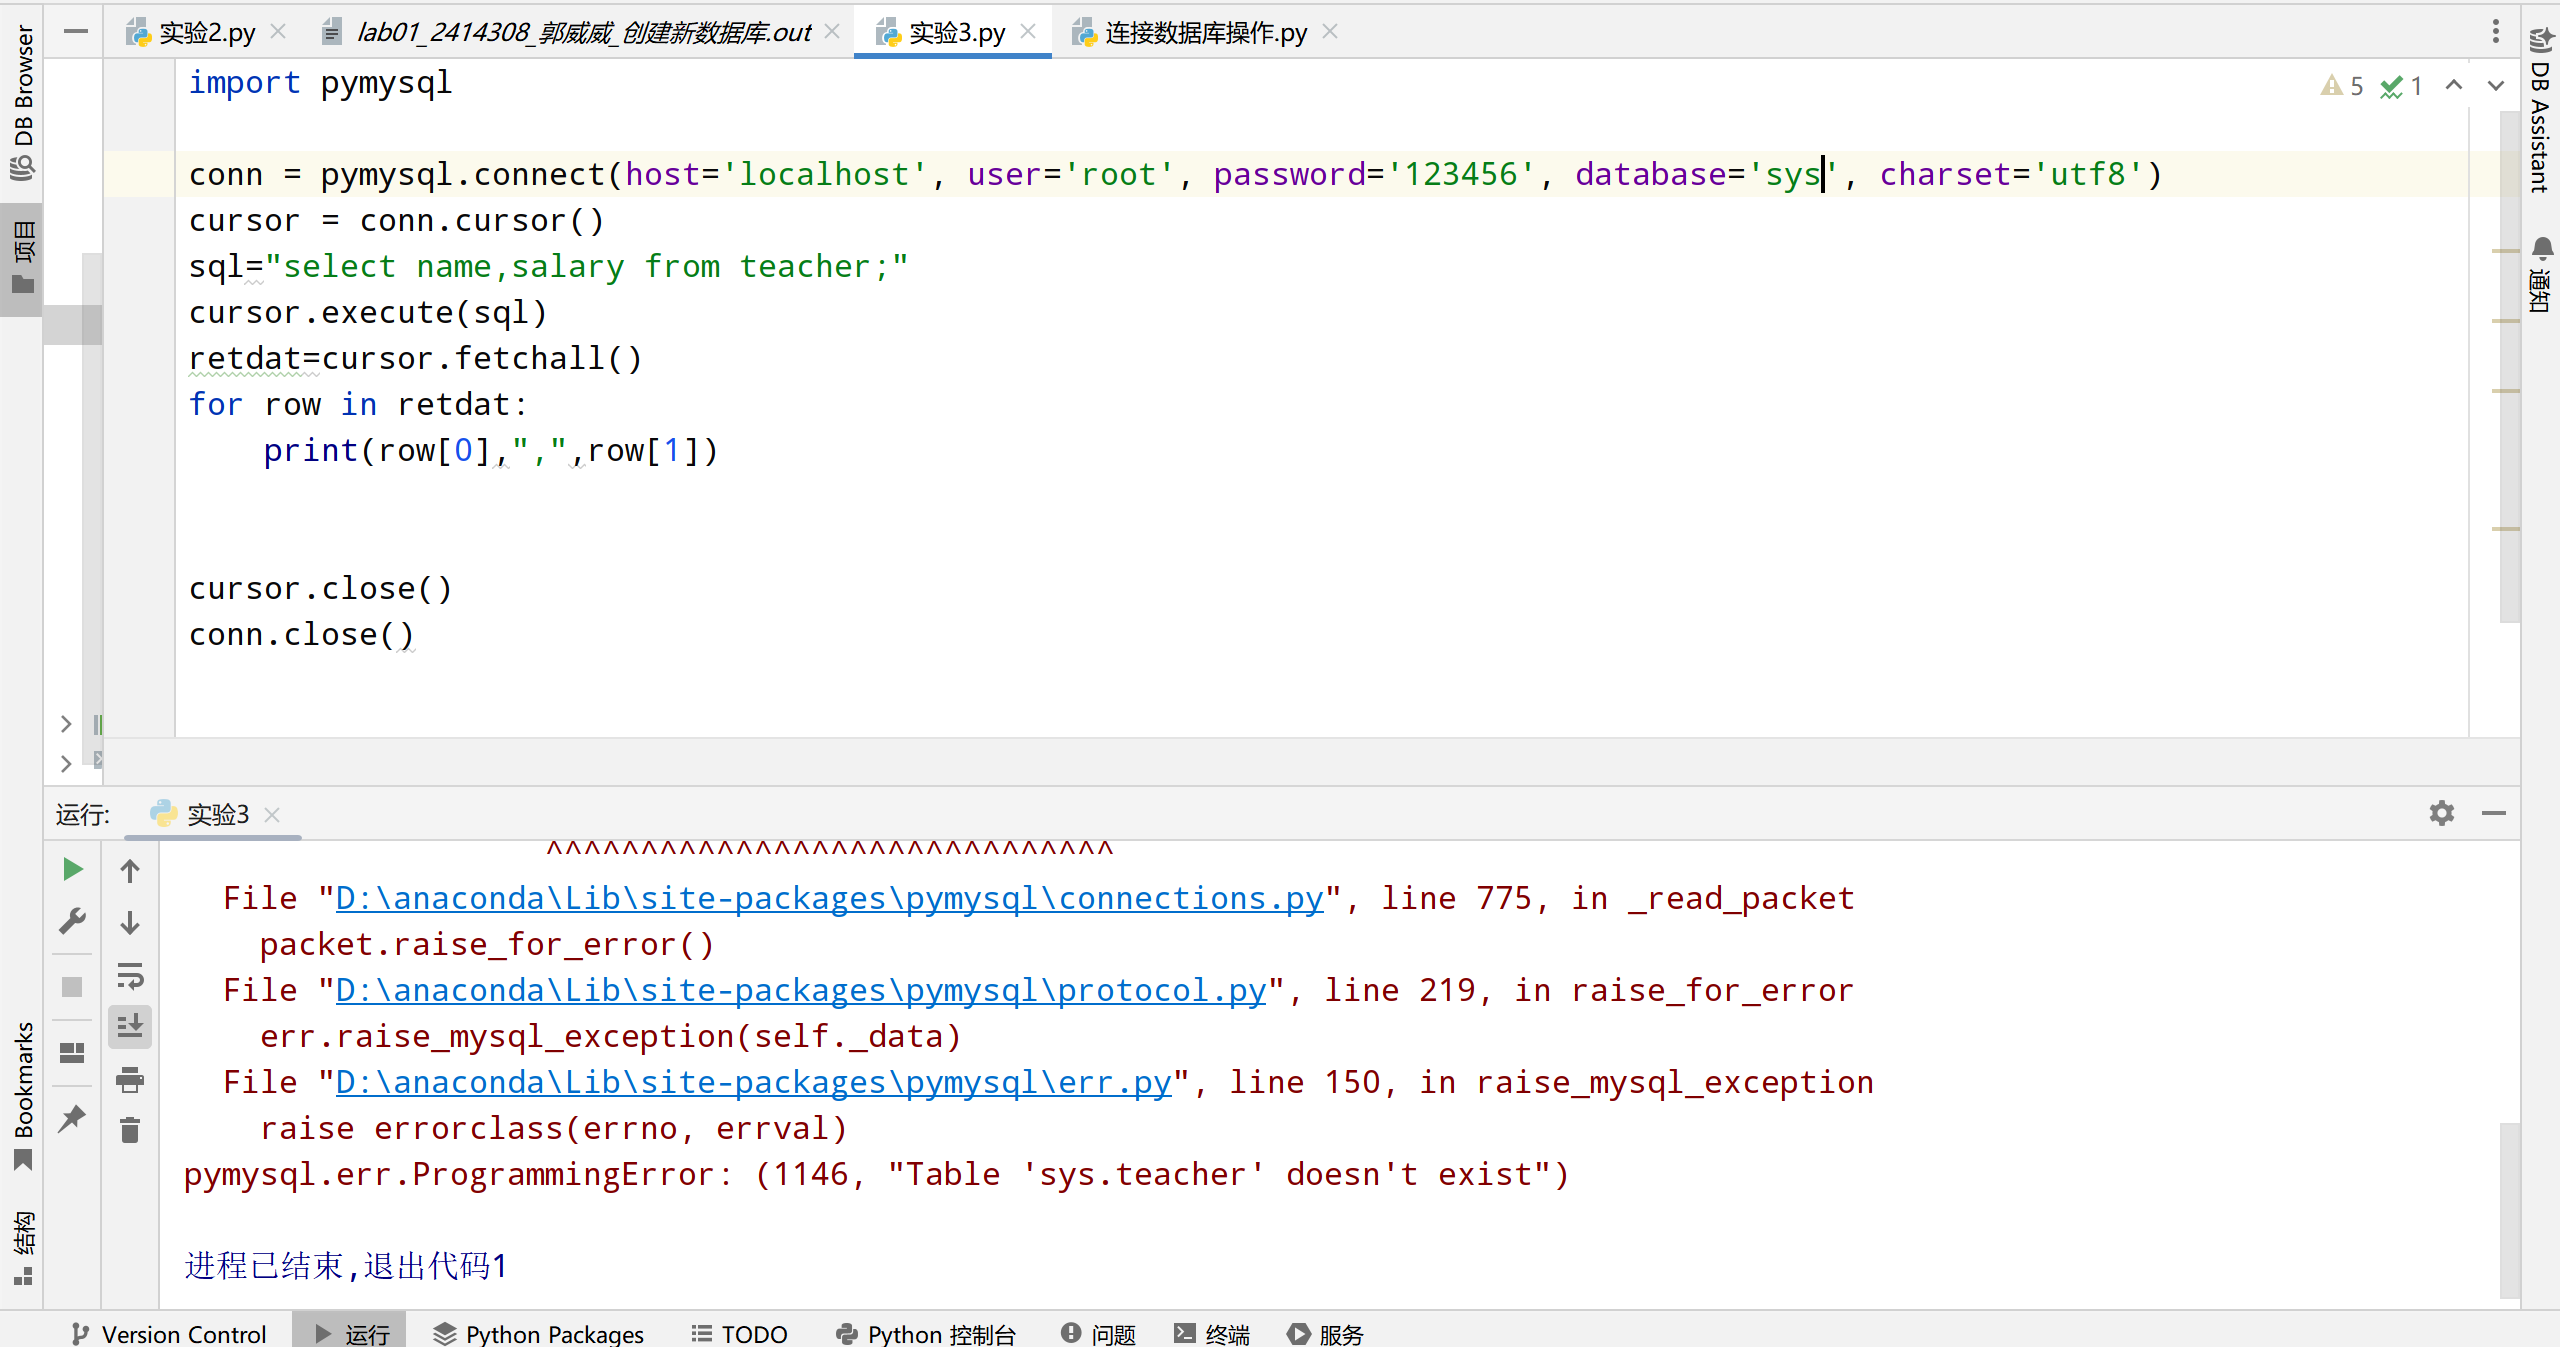
\includegraphics[width=12cm]{figure/image1.png} \\
\footnotesize 图1 软件版本信息截图
\end{center}
\vspace{1cm}

\chapter{实验步骤}
\section{Python环境配置}
1. 安装PyMySQL库：在命令行执行`pip install pymysql`，安装过程中虽有关于`vboxapi`的弃用提示，但成功安装了`PyMySQL-1.1.1`。
2. 测试数据库连接：使用Python代码连接MySQL数据库并查询版本号。
\begin{lstlisting}[language=Python]
import pymysql
conn = pymysql.connect(host='localhost', user='root', password='123456', database='sys', charset='utf8')
cursor = conn.cursor()
sql ='select version()'
cursor.execute(sql)
retdat = cursor.fetchall()
for row in retdat:
    print(row[0])
cursor.close()
conn.close()
\end{lstlisting}
\begin{center}
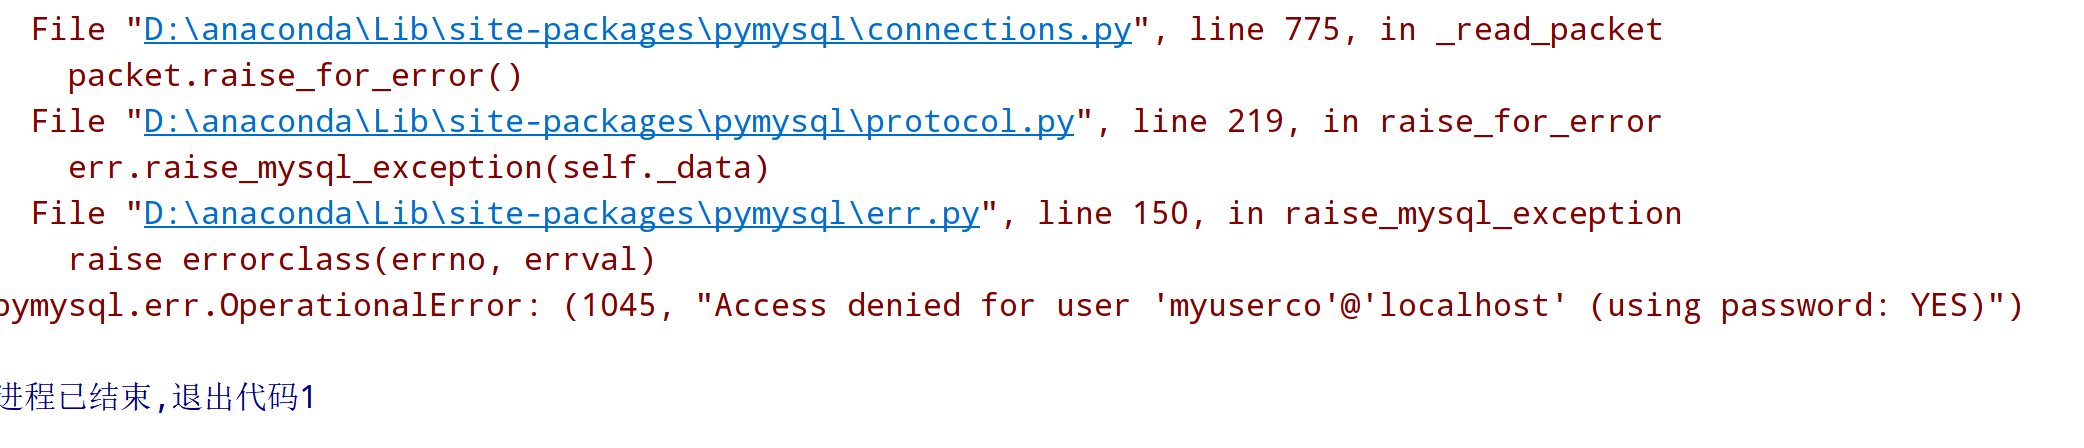
\includegraphics[width=12cm]{figure/image2.png} \\
\footnotesize 图2 Python连接数据库代码截图
\end{center}
\vspace{1cm}
\begin{center}
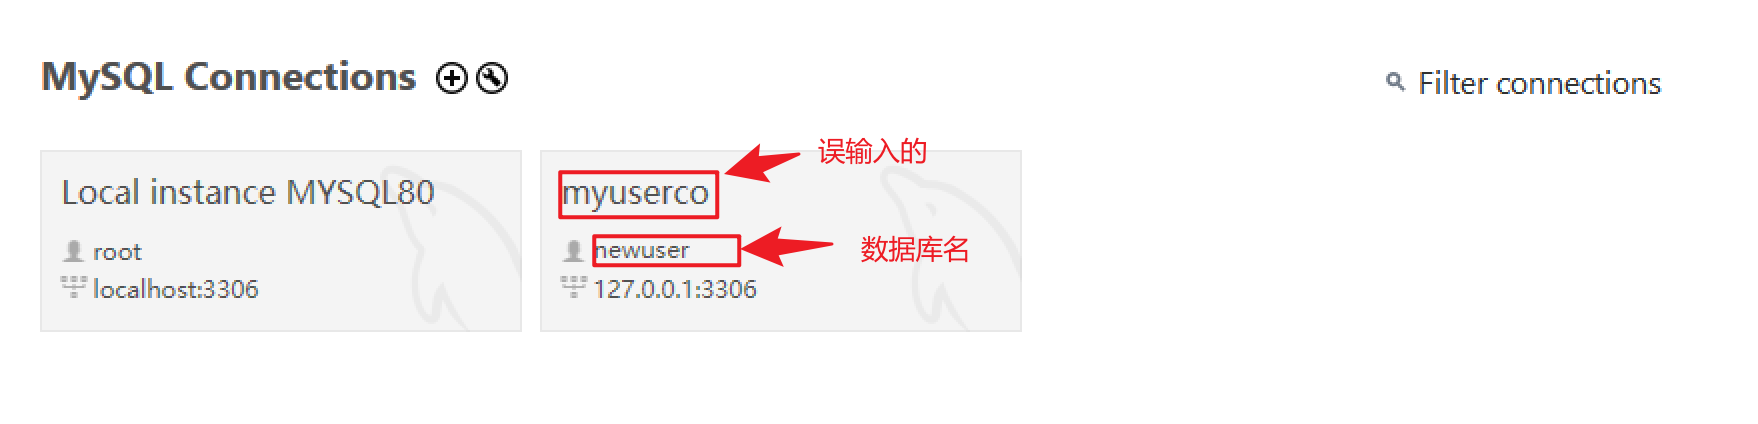
\includegraphics[width=12cm]{figure/image3.png} \\
\footnotesize 图3 Python连接数据库运行结果截图
\end{center}
\vspace{1cm}
运行结果显示MySQL版本为8.0.41，表明连接成功。

\section{创建新用户并授权用户权限}
1. 创建用户：在MySQL Workbench的“Administration - Users and Privileges”中，添加新用户`newuser`，设置密码，选择主机为`%`以允许远程访问。
2. 授权权限：授予`newuser`所有权限，包括管理、数据操作等，点击“Apply”完成设置。
\begin{center}
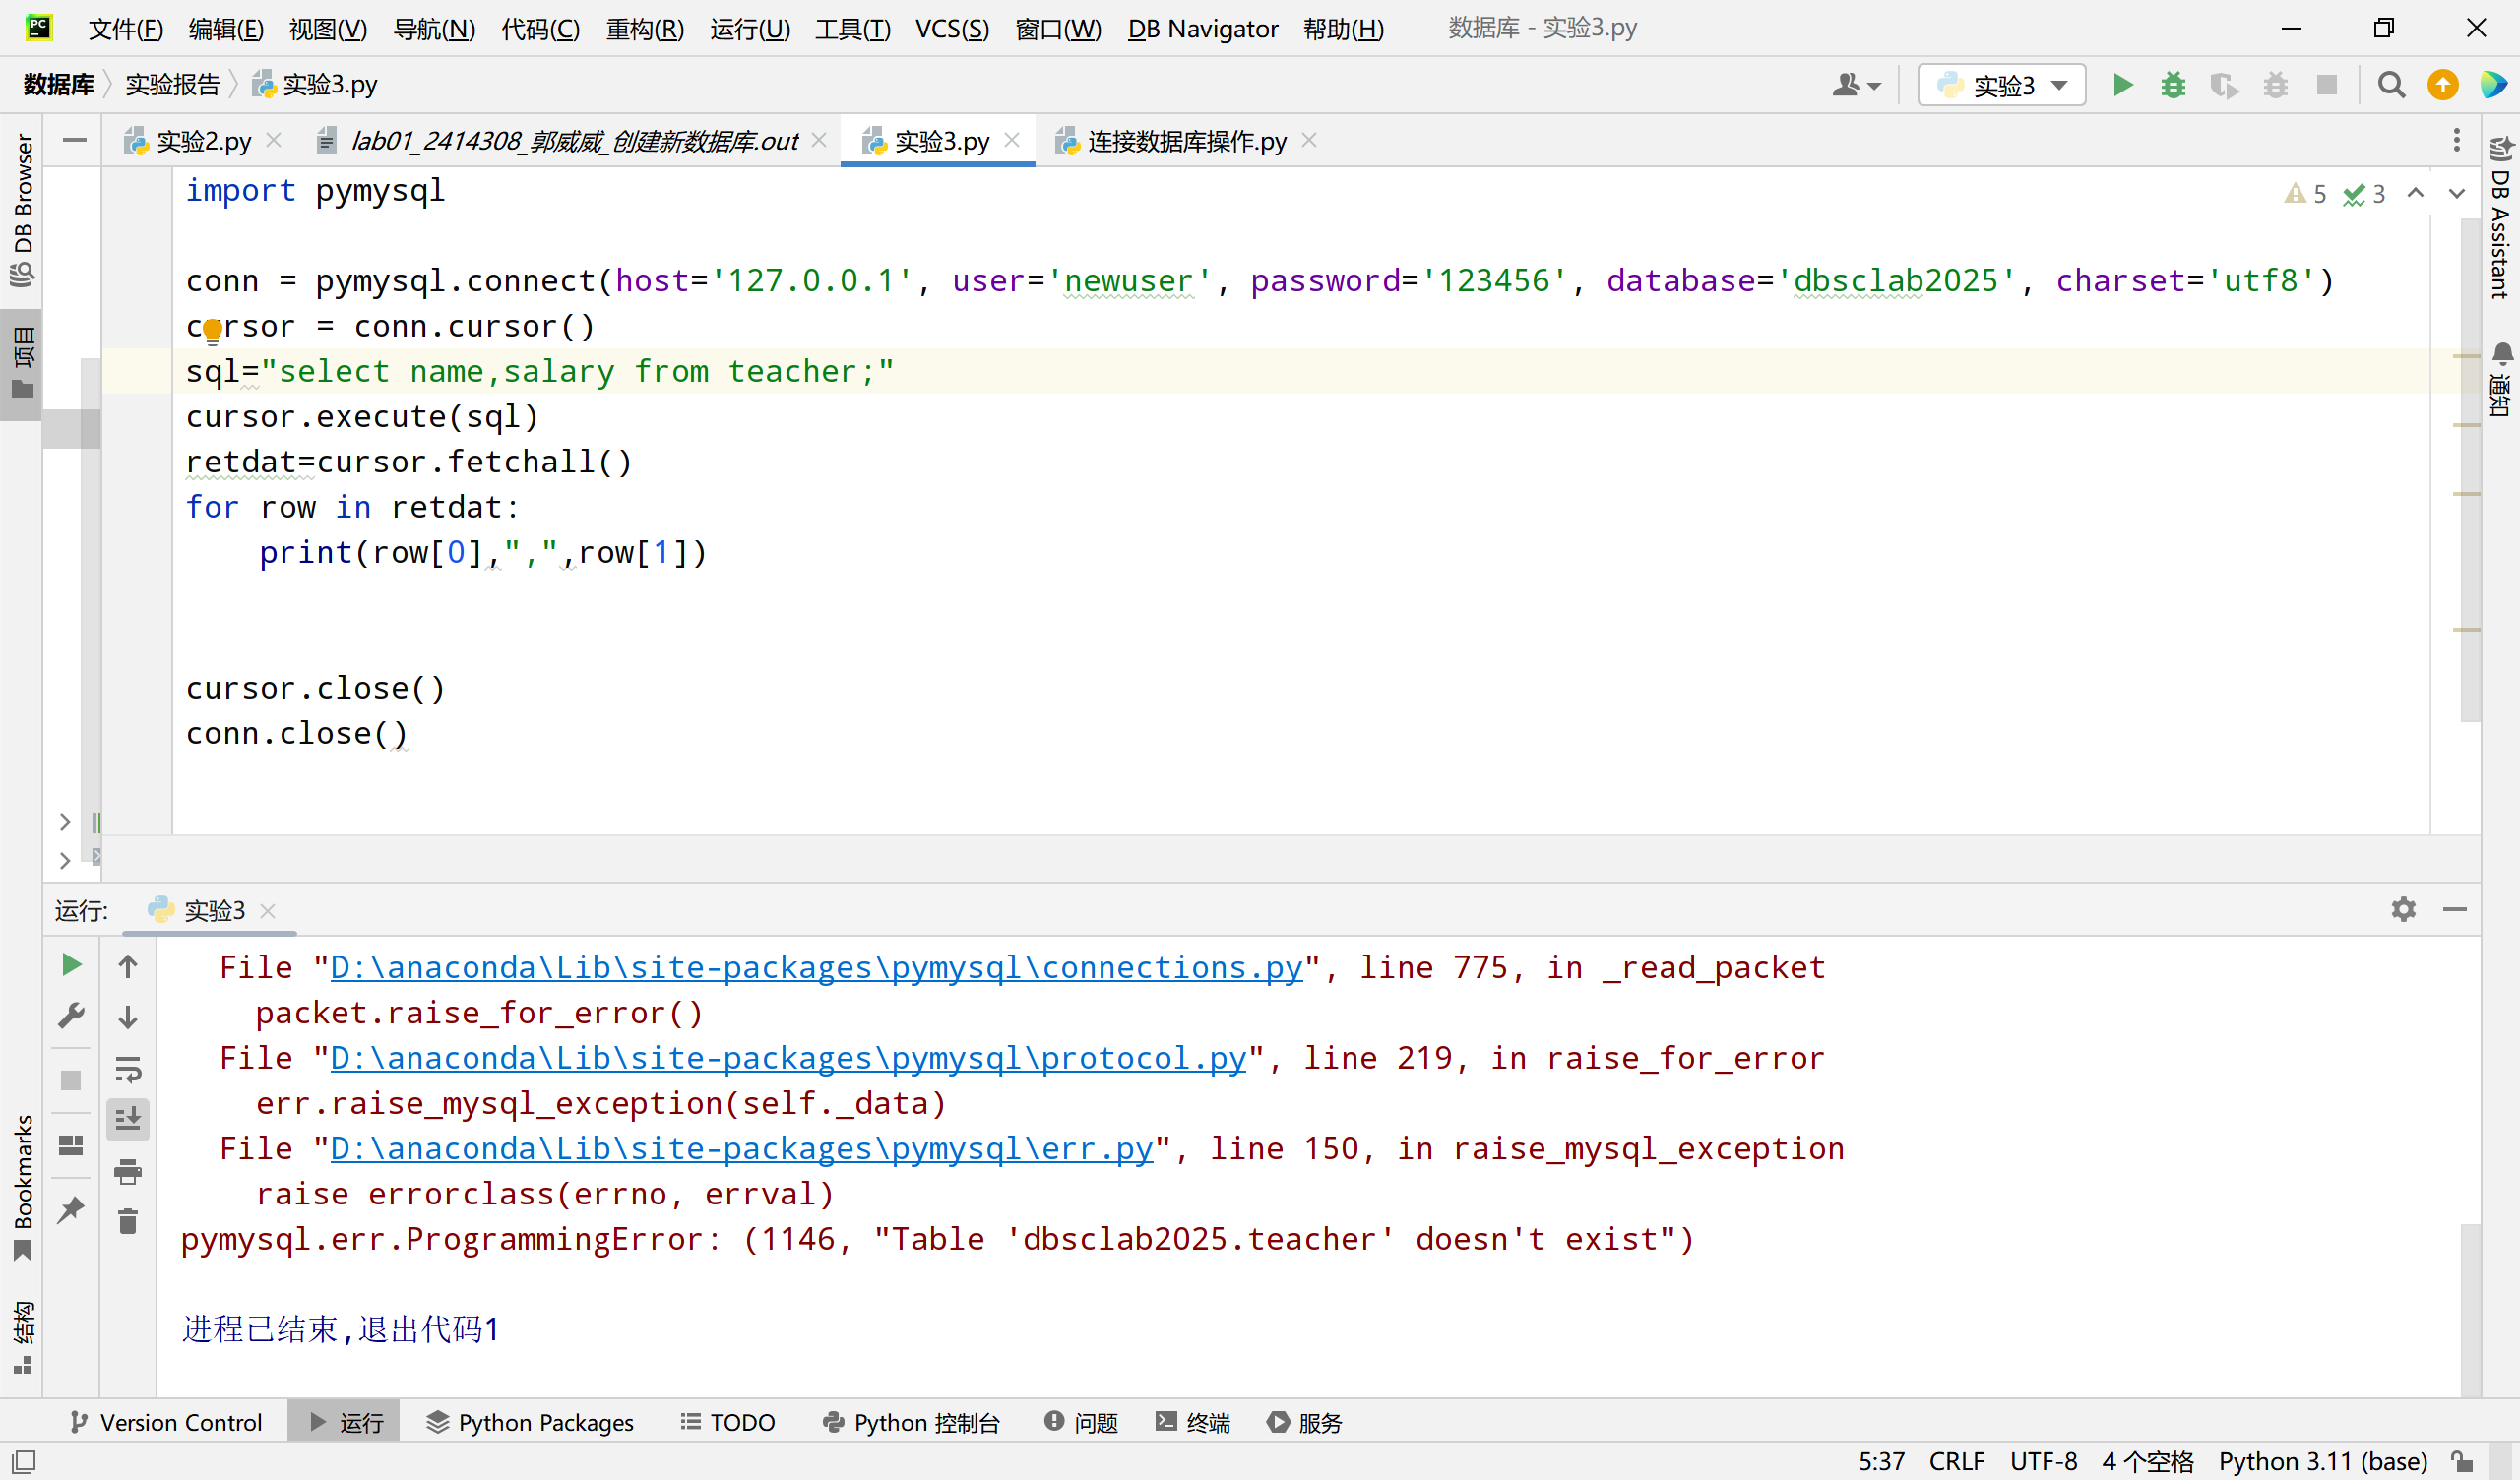
\includegraphics[width=12cm]{figure/image4.png} \\
\footnotesize 图4 创建新用户界面截图
\end{center}
\vspace{1cm}
\begin{center}
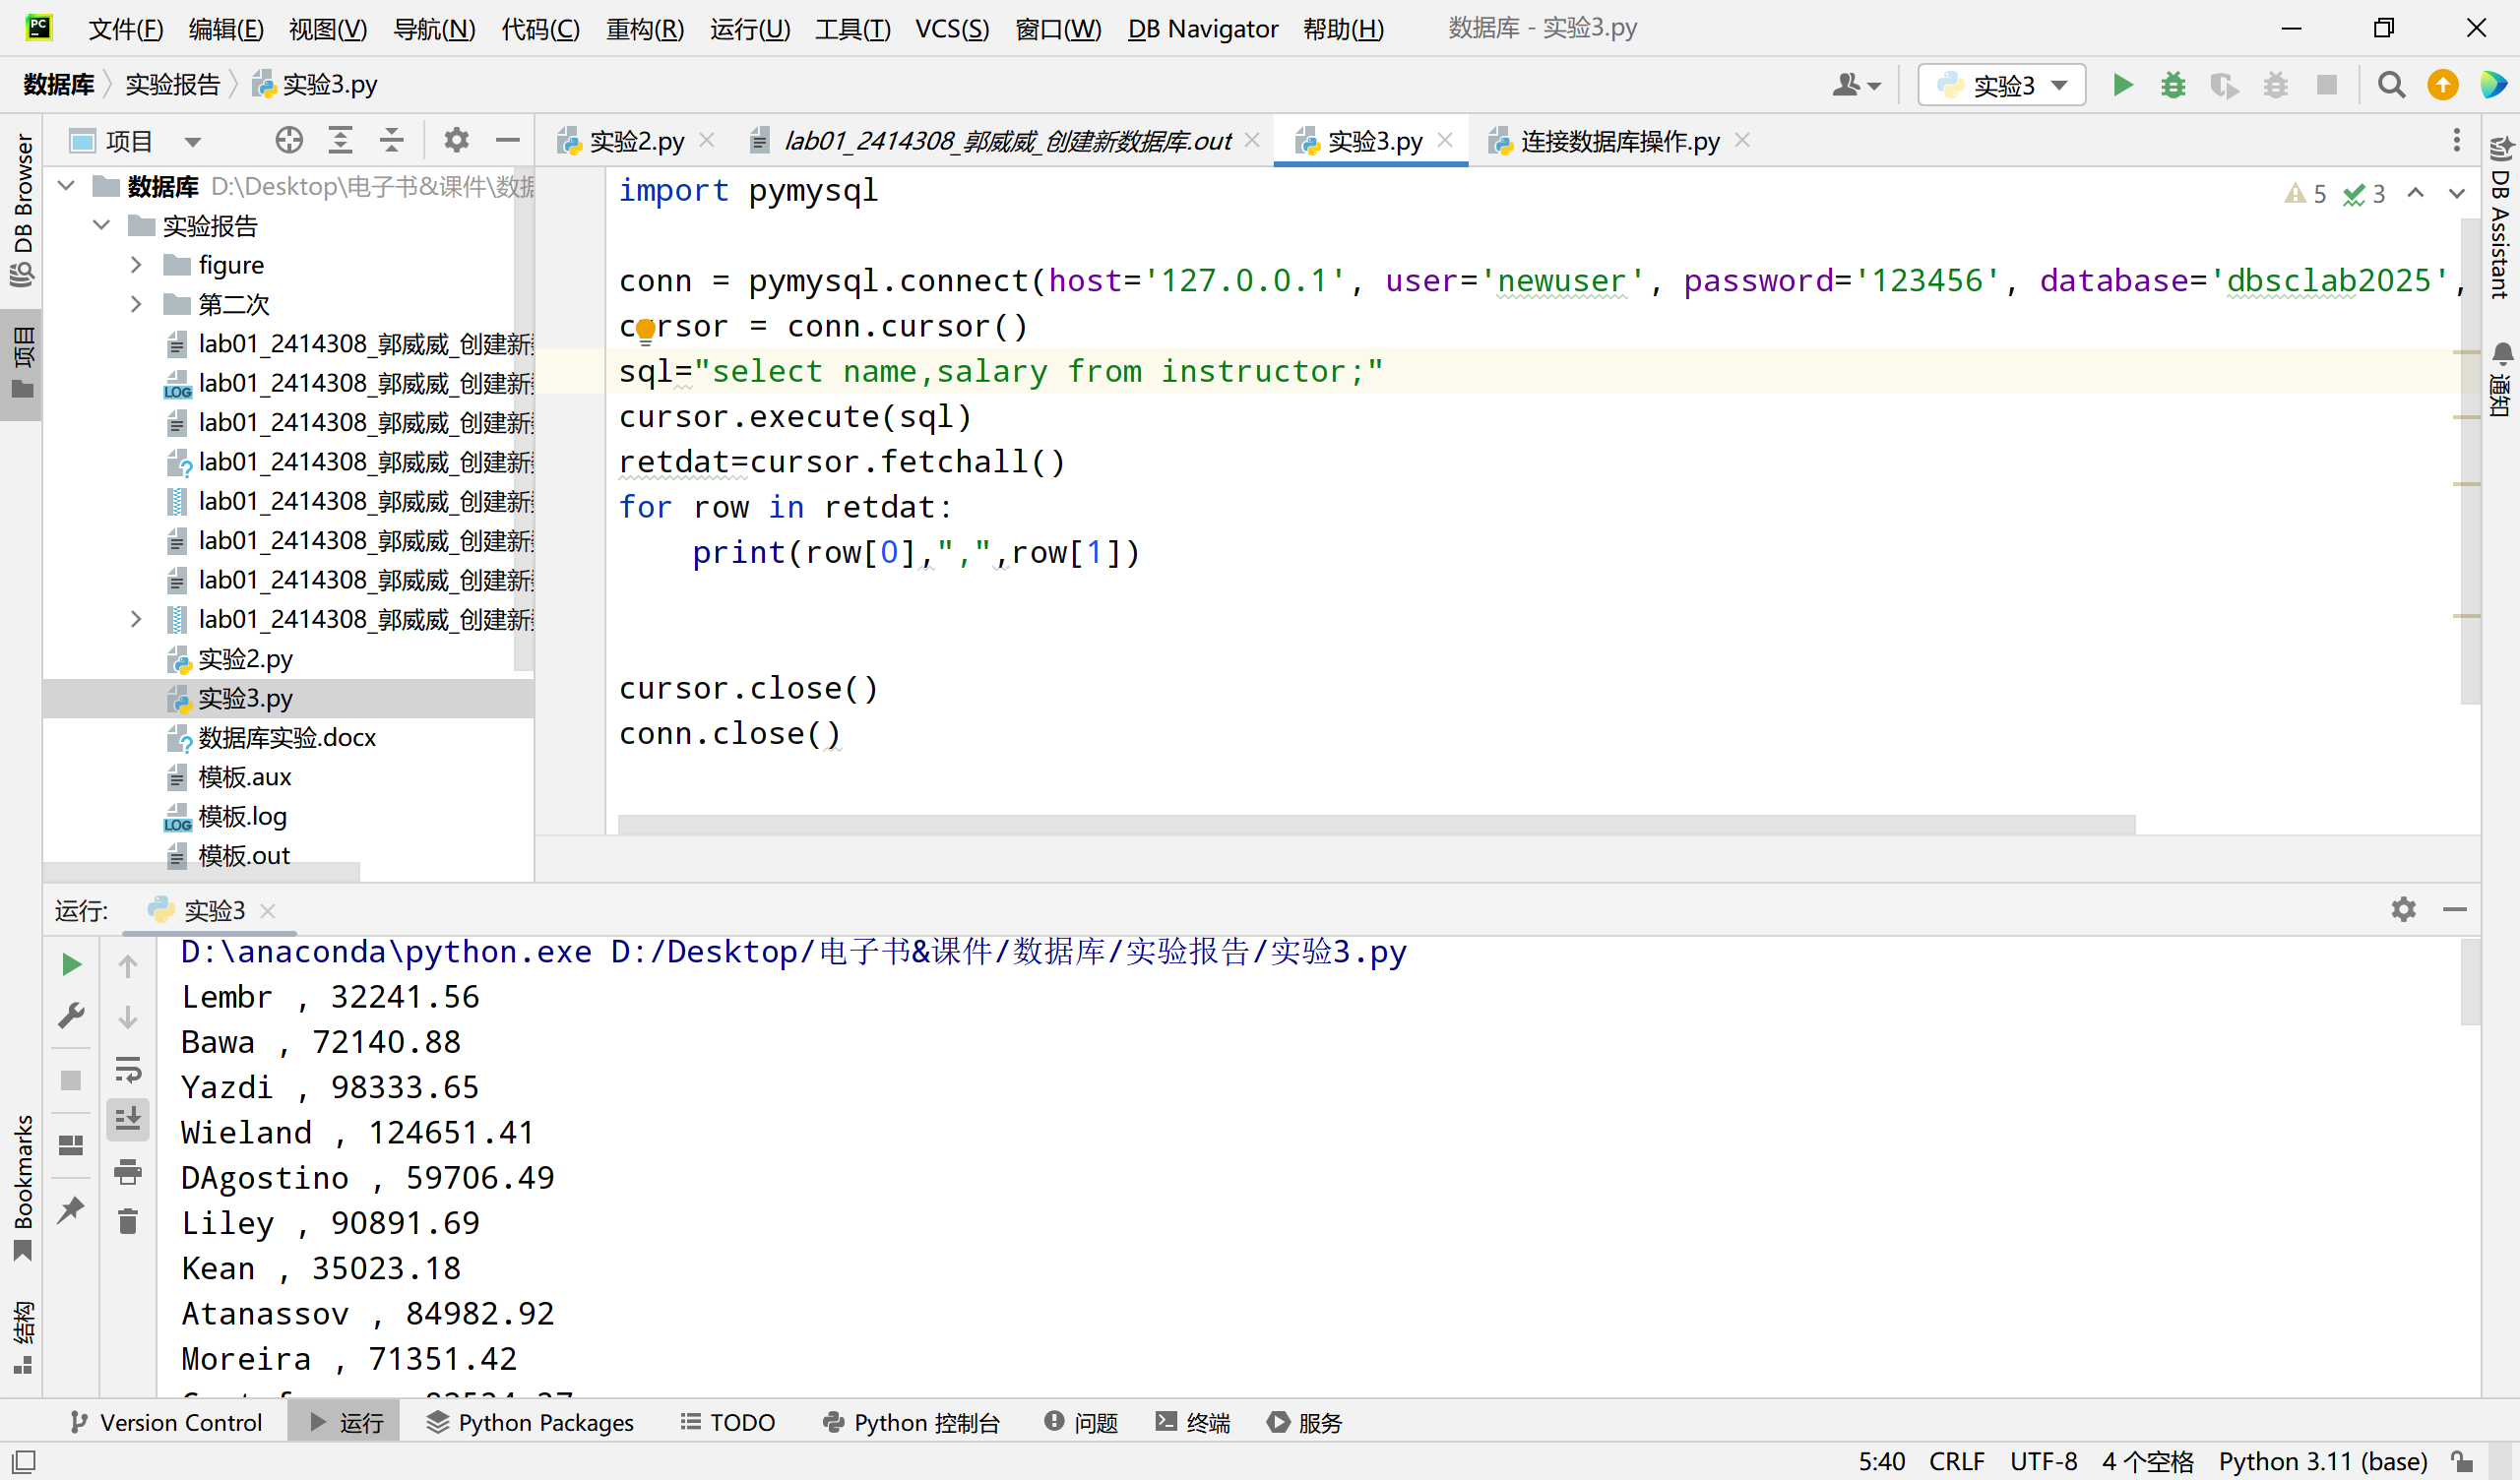
\includegraphics[width=12cm]{figure/image5.png} \\
\footnotesize 图5 授权用户权限界面截图
\end{center}
\vspace{1cm}

\section{创建新数据库并导入模板}
1. 创建数据库：在MySQL Workbench的“Navigator”面板，右键点击“Schemas”，选择“Create Schema”，输入数据库名`dbsclab2025`，设置字符集和排序规则后点击“Apply”。
2. 导入模板：点击“Navigator”面板中的“Data Import/Restore”，选择“Import from Self-Contained File”，指定模板文件路径，选择目标数据库`dbsclab2025`，点击“Start Import”完成导入。期间因用户名输入错误导致连接问题，修正后成功导入。
\begin{center}
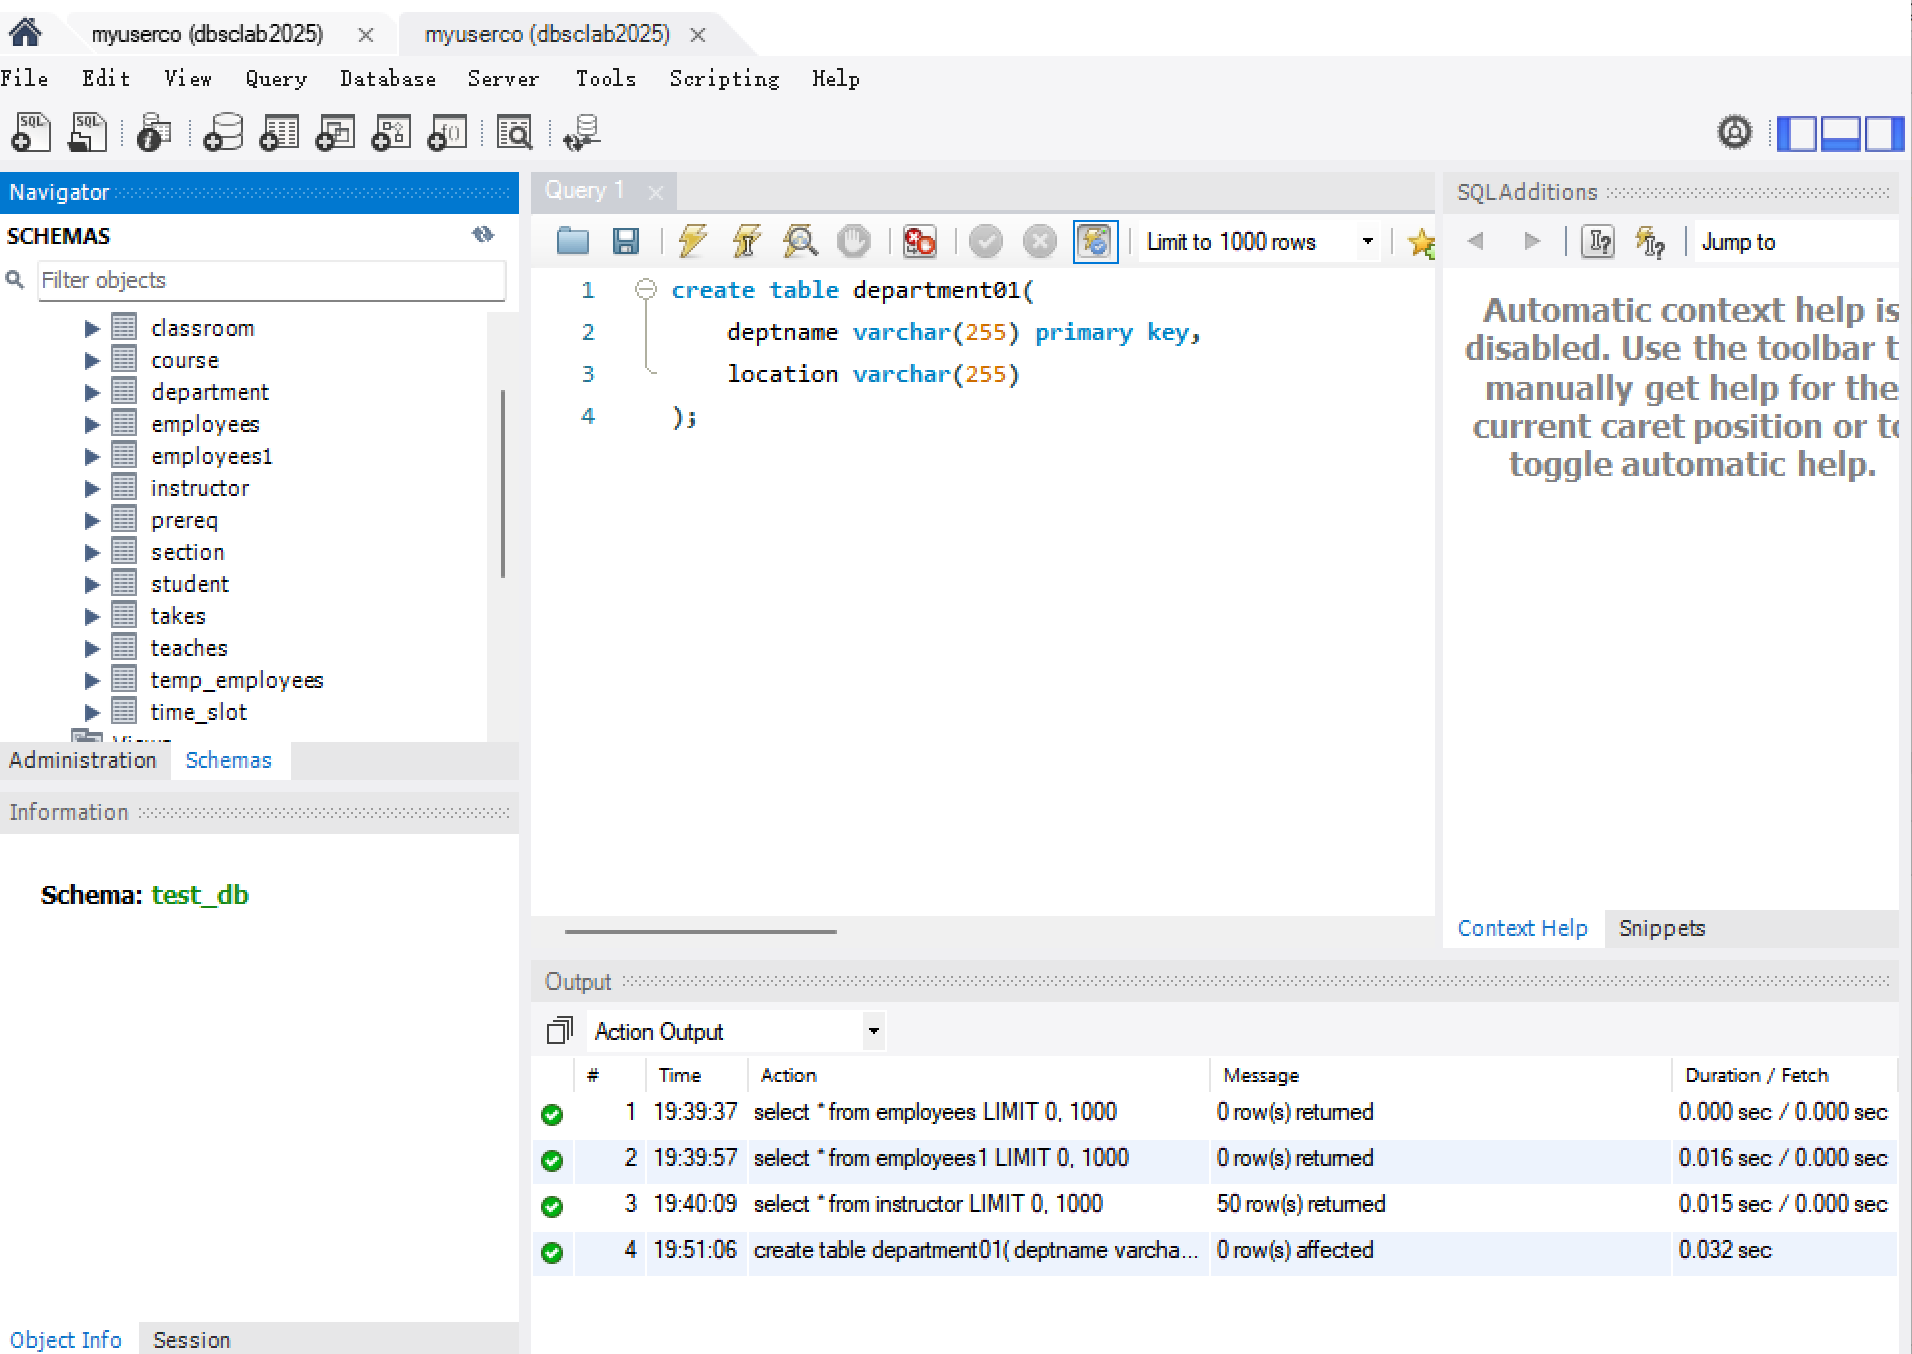
\includegraphics[width=12cm]{figure/image6.png} \\
\footnotesize 图6 创建数据库界面截图
\end{center}
\vspace{1cm}
配置后输入密码错误，没找到结果发现用户名输入错了
\begin{center}
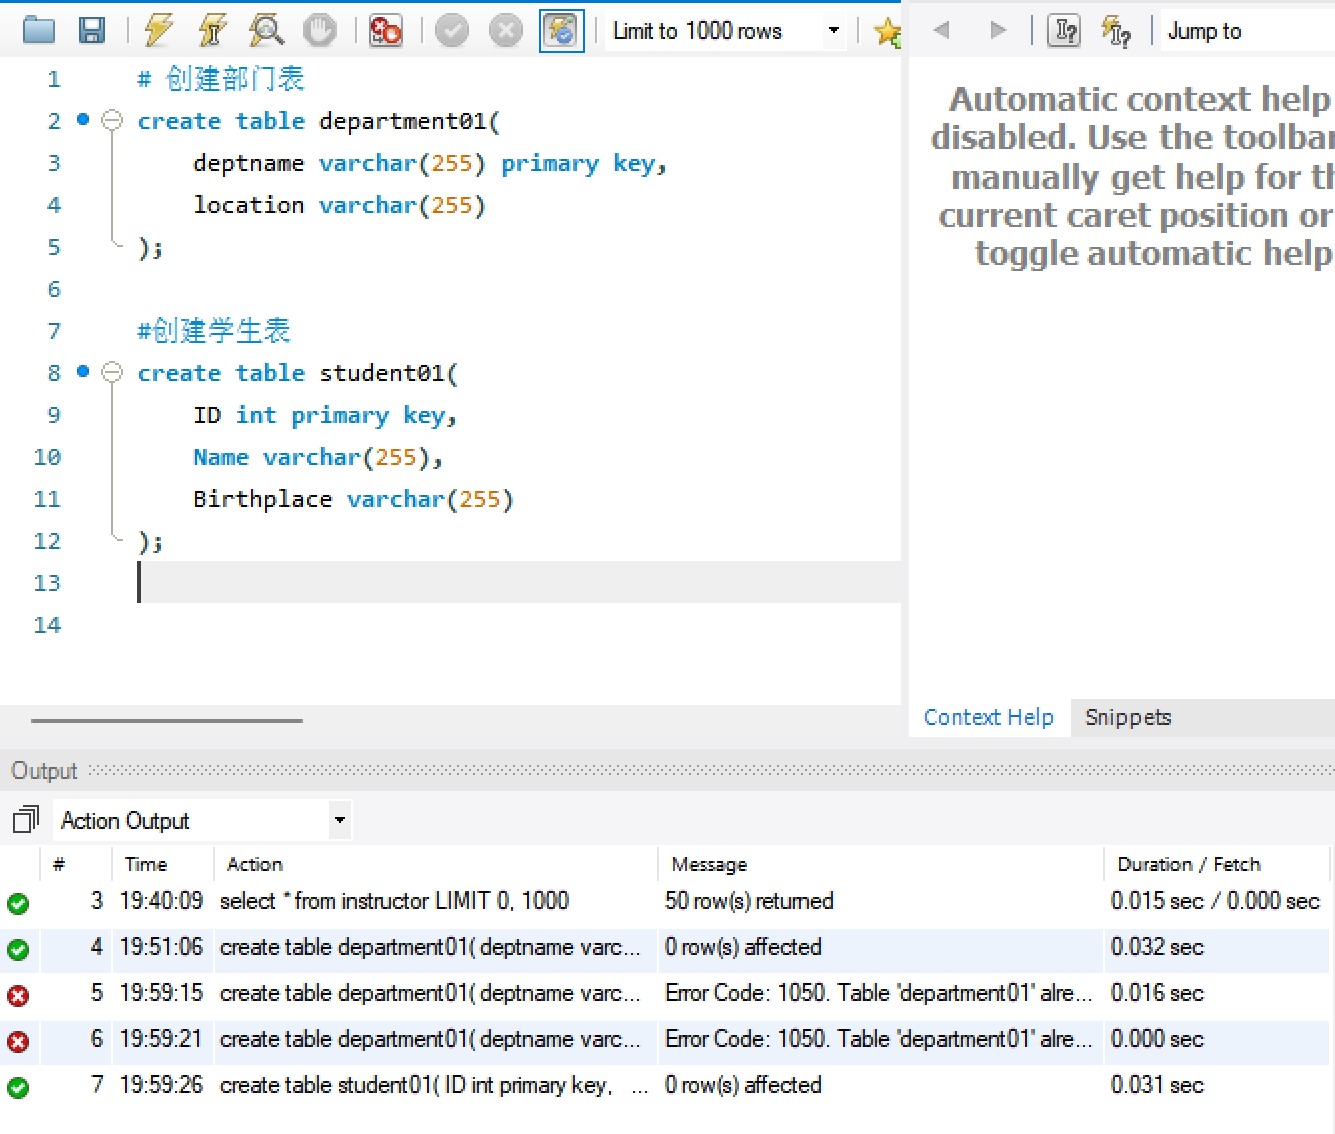
\includegraphics[width=12cm]{figure/image7.png} \\
\footnotesize 图7 配置数据库连接界面截图（错误情况）
\end{center}
\vspace{1cm}
设置完成后主页没显示，退出重启后显示结果
\begin{center}
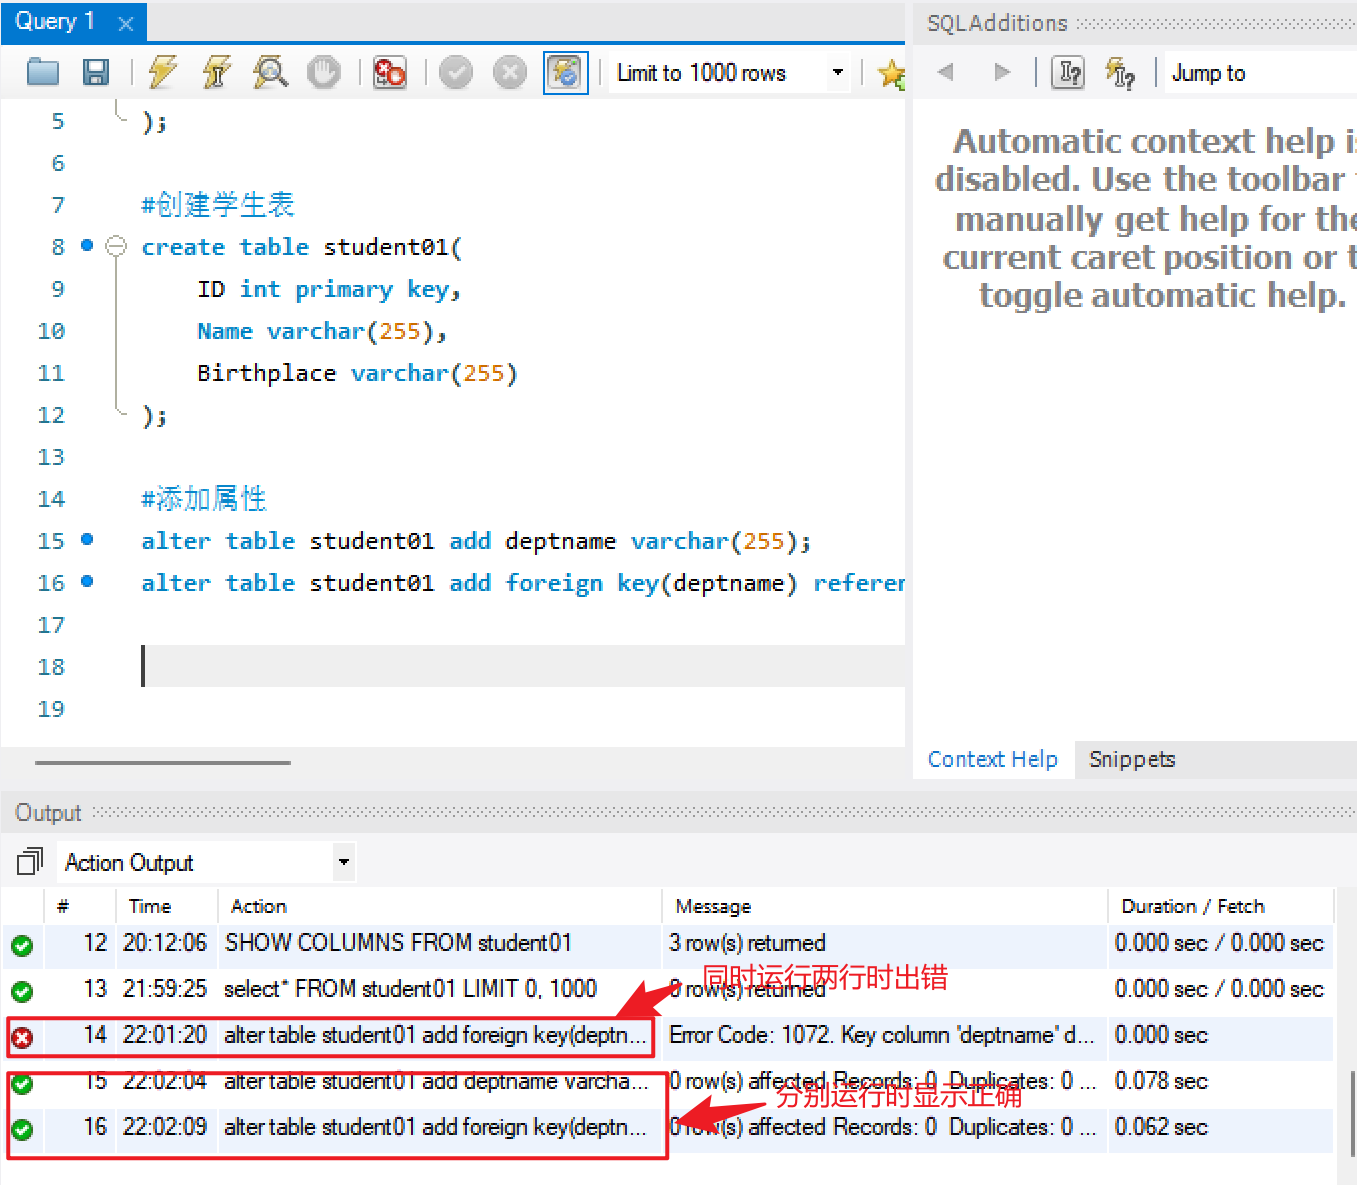
\includegraphics[width=12cm]{figure/image8.png} \\
\footnotesize 图8 数据库显示结果界面截图
\end{center}
\vspace{1cm}
创建新模板
\begin{center}
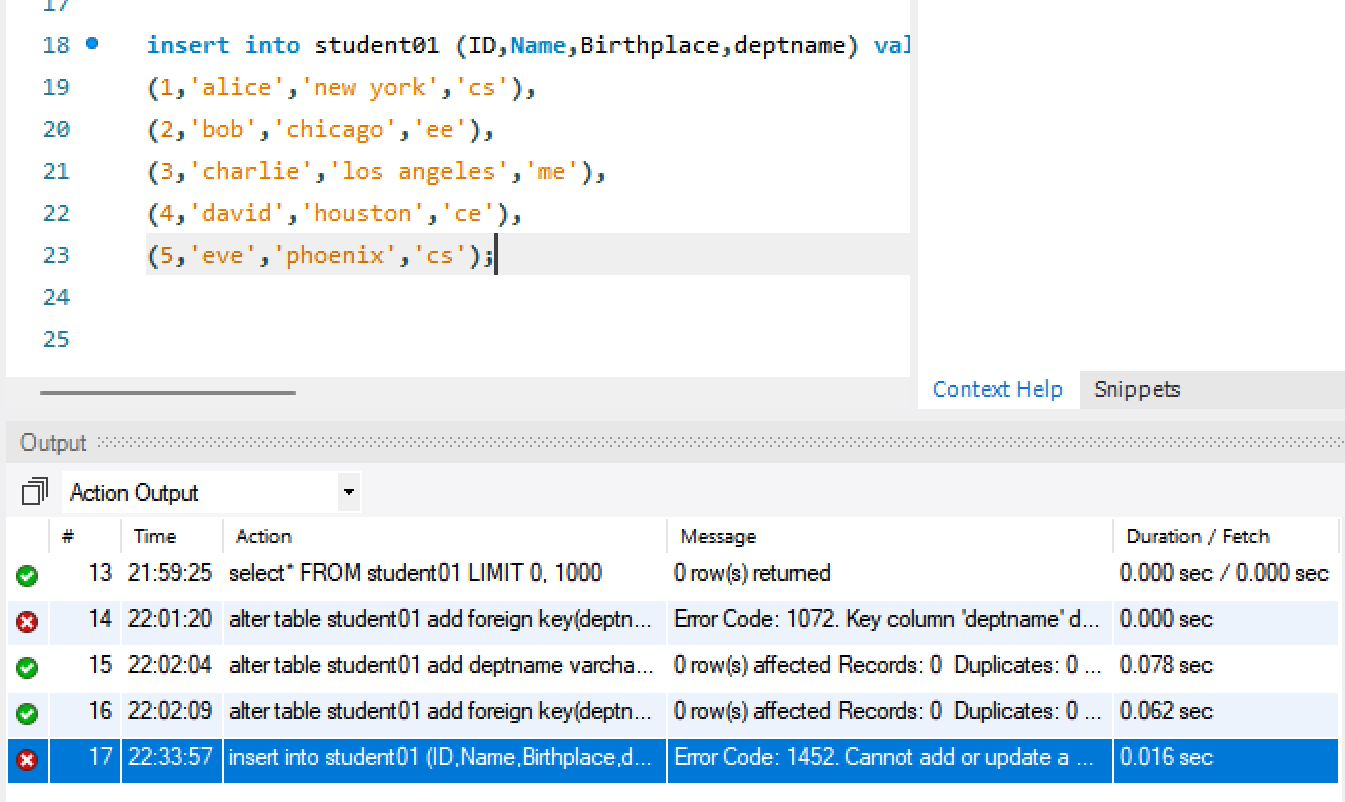
\includegraphics[width=12cm]{figure/image9.png} \\
\footnotesize 图9 创建新模板相关界面截图1
\end{center}
\vspace{1cm}
\begin{center}
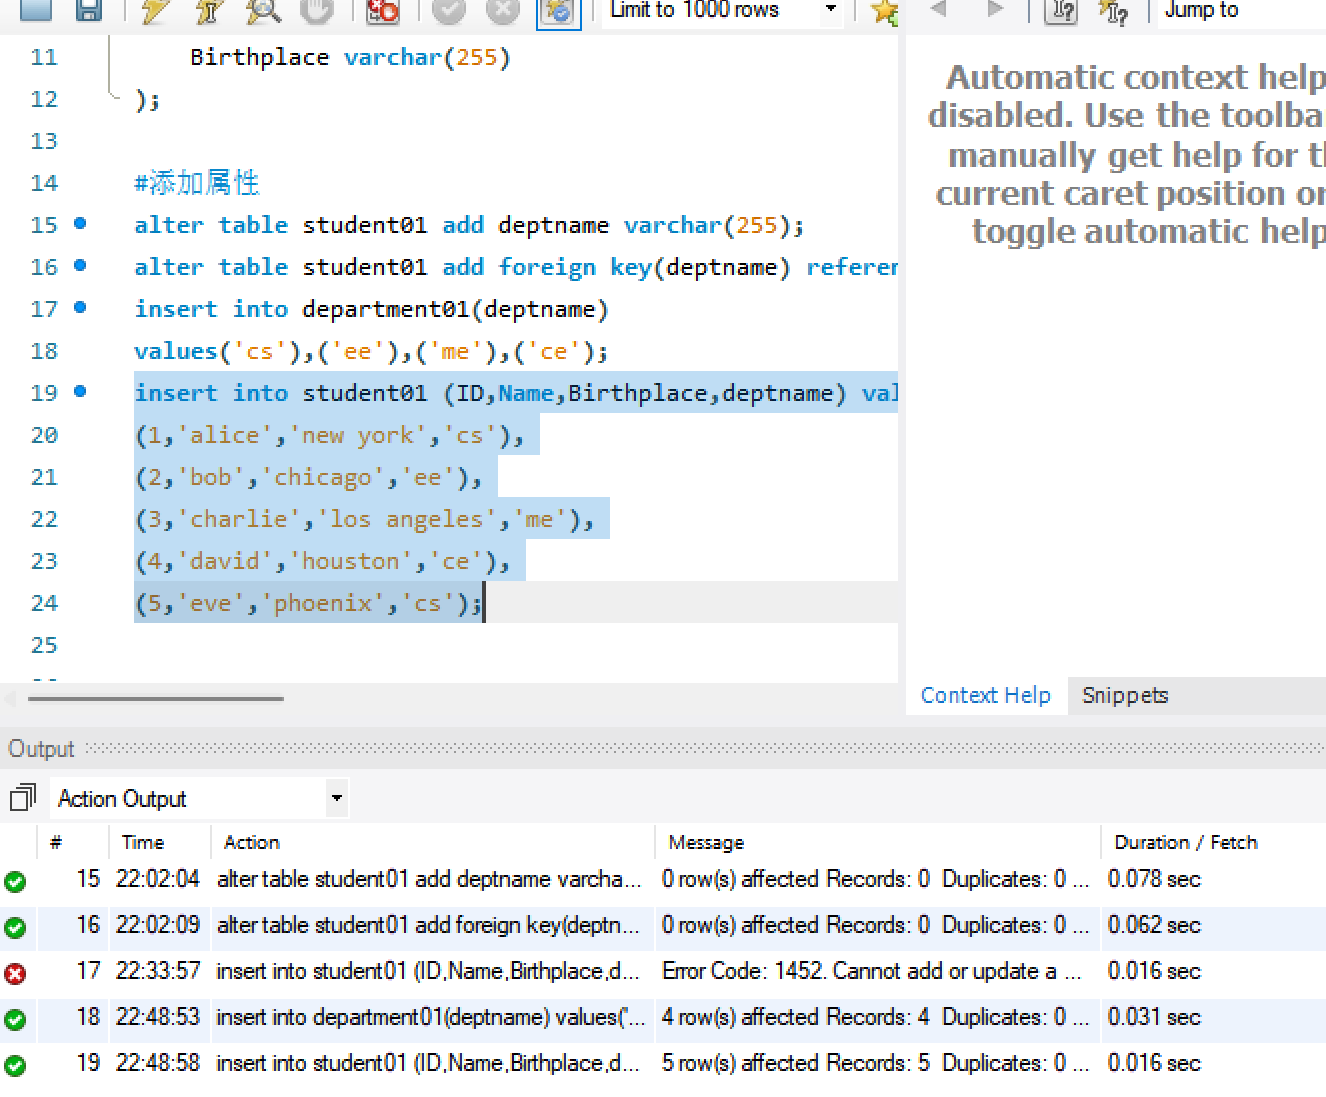
\includegraphics[width=12cm]{figure/image10.png} \\
\footnotesize 图10 创建新模板相关界面截图2
\end{center}
\vspace{1cm}
\begin{center}
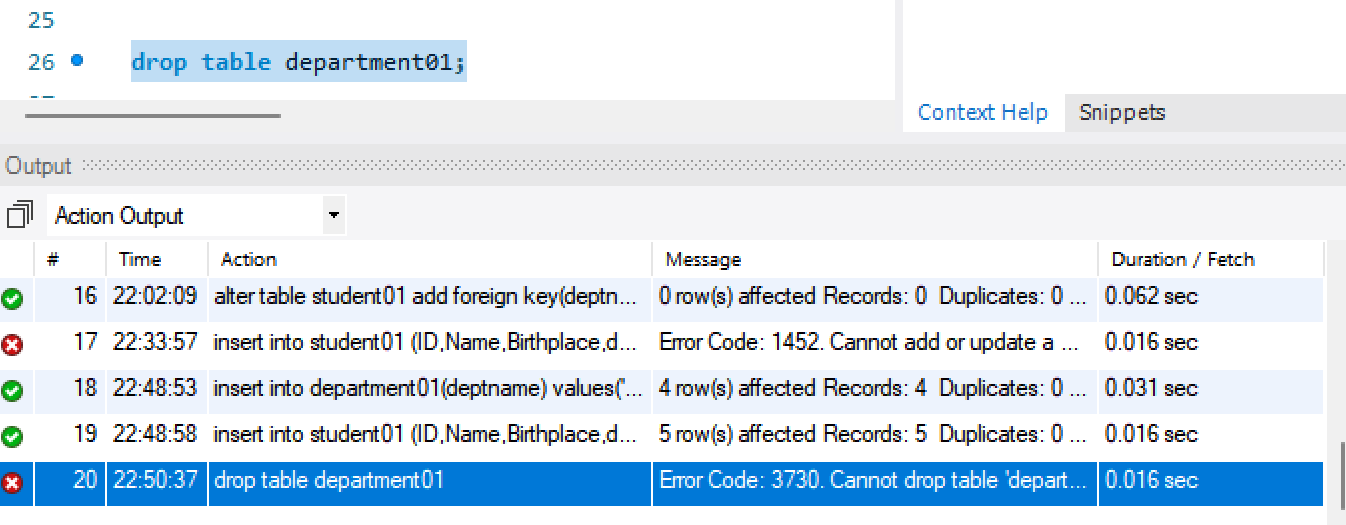
\includegraphics[width=12cm]{figure/image11.png} \\
\footnotesize 图11 创建新模板相关界面截图3
\end{center}
\vspace{1cm}

\section{创建表}
在MySQL Workbench的查询窗口，针对`dbsclab2025`数据库执行建表语句，如创建`stu`表。
\begin{lstlisting}[language=SQL]
CREATE TABLE stu (
    id varchar(18),
    name varchar(18),
    age int
);
insert into stu values('123', 'xiaoming',18);
select * from stu;
\end{lstlisting}
\begin{center}
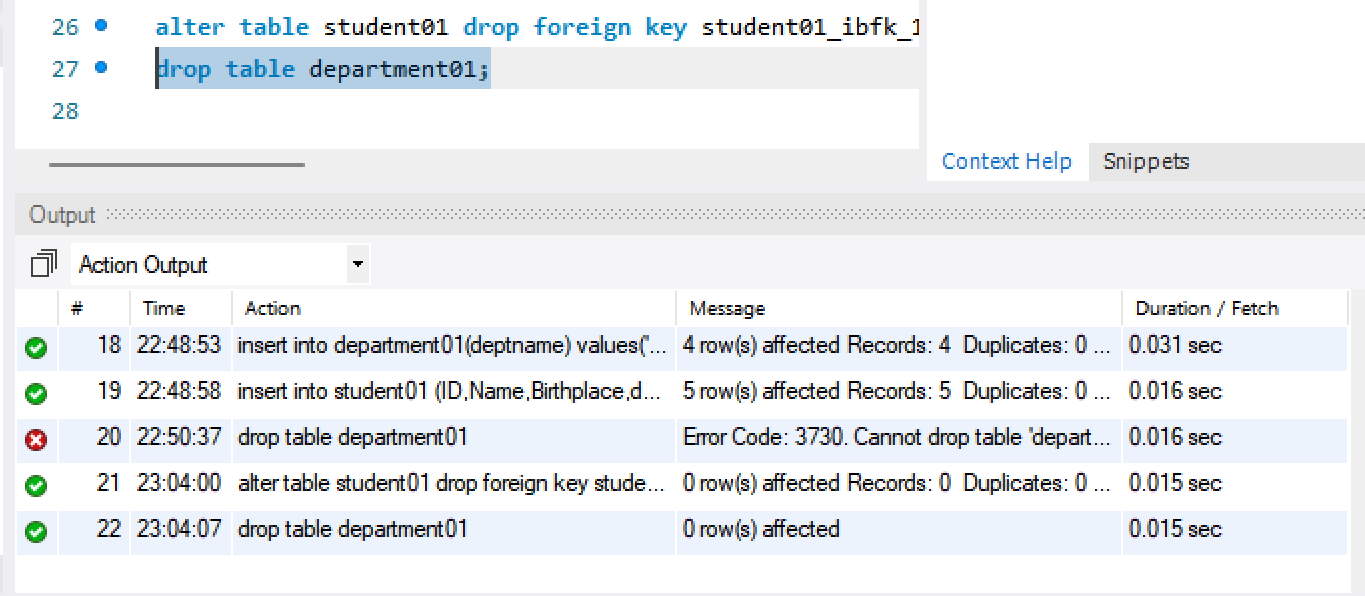
\includegraphics[width=12cm]{figure/image12.png} \\
\footnotesize 图12 创建stu表及操作截图
\end{center}
\vspace{1cm}

\subsection{简单查询声明}
% 此处列出多个查询语句，根据实际情况，若有对应图片，可在相应位置插入
\begin{lstlisting}[language=SQL]
drop table if exists prereq;
drop table if exists time_slot;
drop table if exists advisor;
drop table if exists takes;
drop table if exists student;
drop table if exists teaches;
drop table if exists section;
drop table if exists instructor;
drop table if exists course;
drop table if exists department;
drop table if exists classroom;
create table classroom (
    building varchar(15),
    room_number varchar(7)
);
\end{lstlisting}
\begin{center}
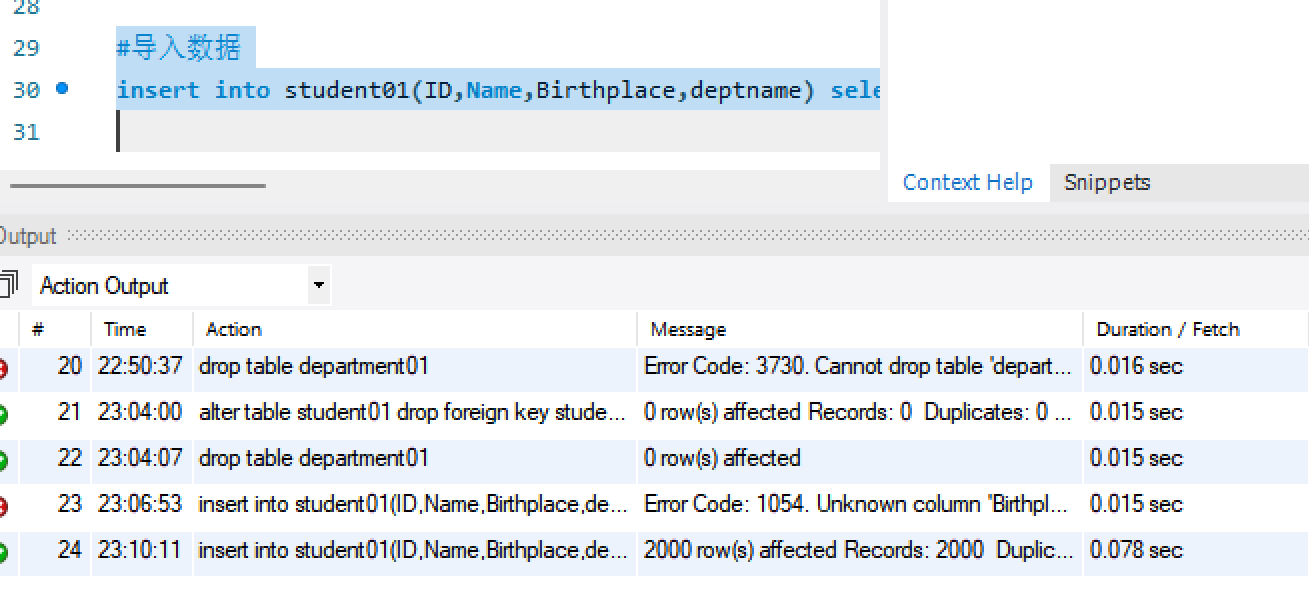
\includegraphics[width=12cm]{figure/image13.png} \\
\footnotesize 图13 简单查询声明相关操作截图1
\end{center}
\vspace{1cm}
% 其他查询语句类似处理，如：
\begin{lstlisting}[language=SQL]
use dbsclab2025;
select ID, name, dept_name from instructor;
select * from department;
select dept_name, budget from department;
-- 原文档中错误语句已修正，此处保留正确逻辑
select * from student where dept_name='History';
\end{lstlisting}
\begin{center}
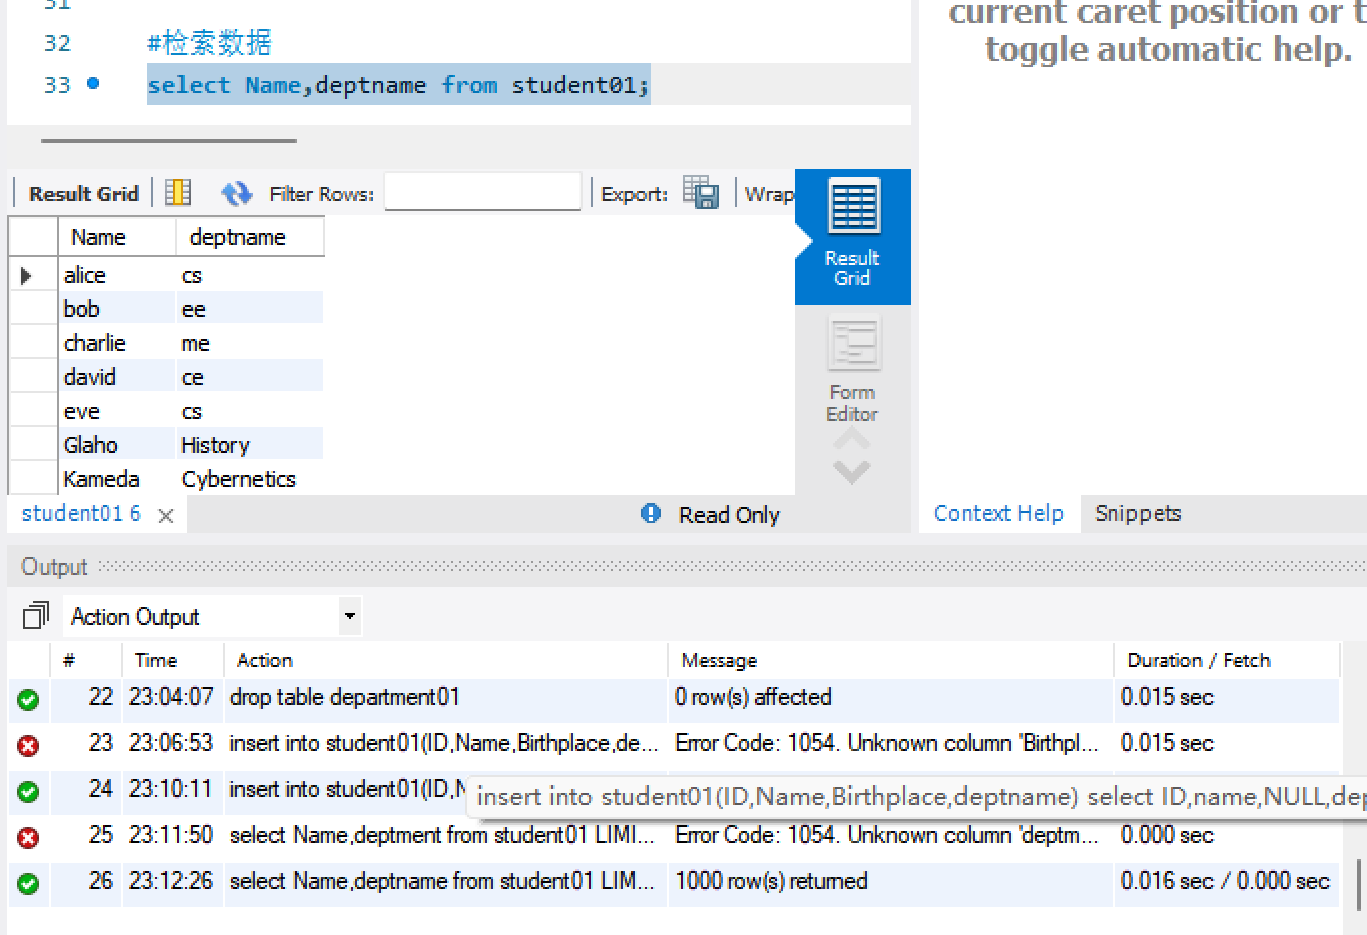
\includegraphics[width=12cm]{figure/image14.png} \\
\footnotesize 图14 简单查询声明相关操作截图2
\end{center}
\vspace{1cm}
\begin{center}
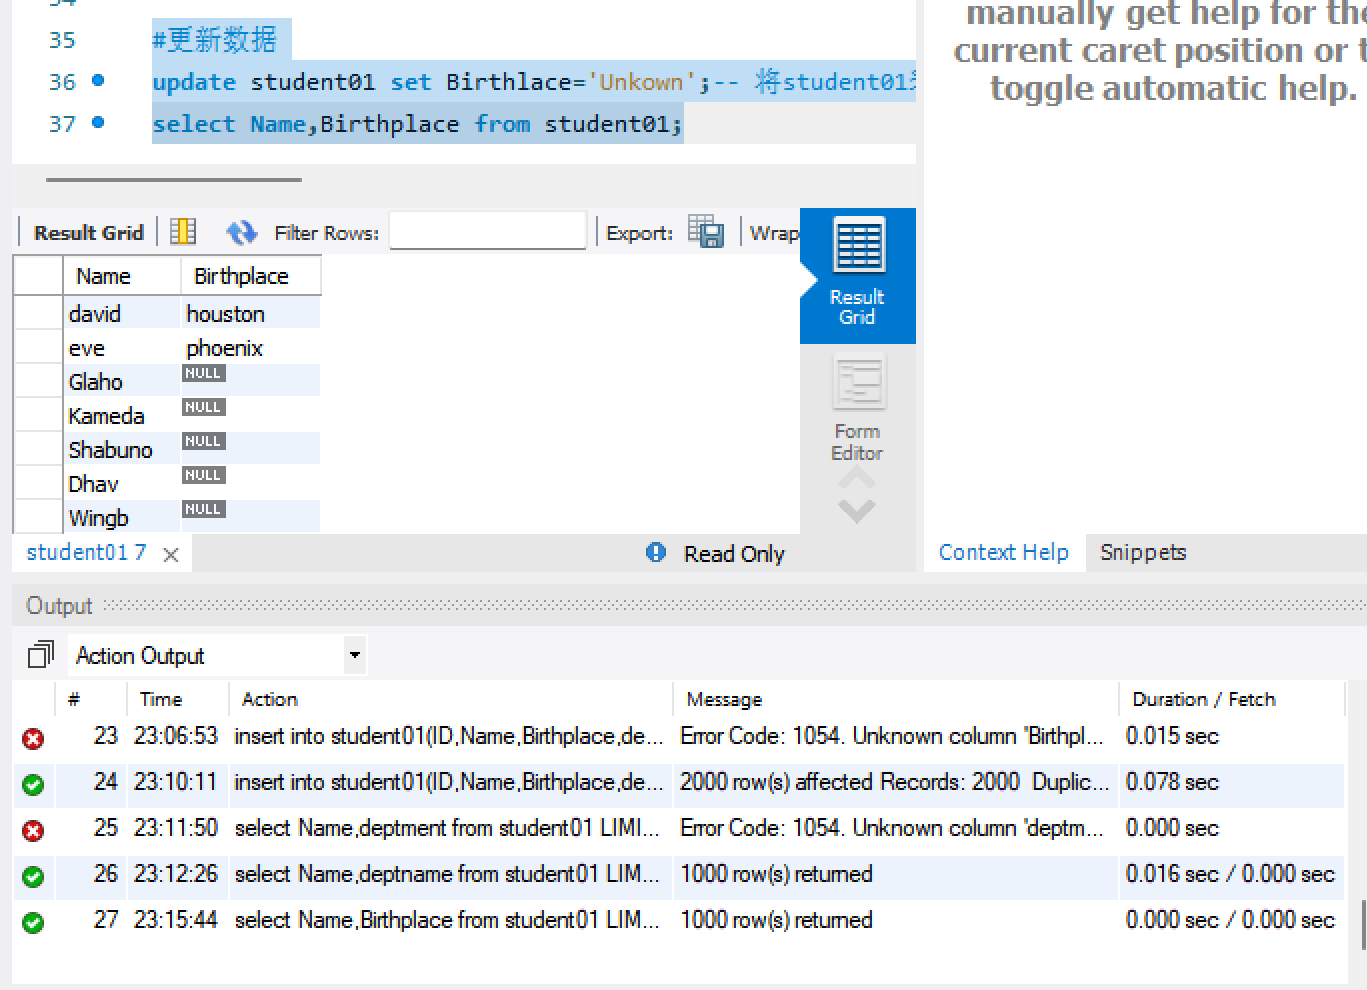
\includegraphics[width=12cm]{figure/image15.png} \\
\footnotesize 图15 简单查询声明相关操作截图3
\end{center}
\vspace{1cm}
\begin{center}
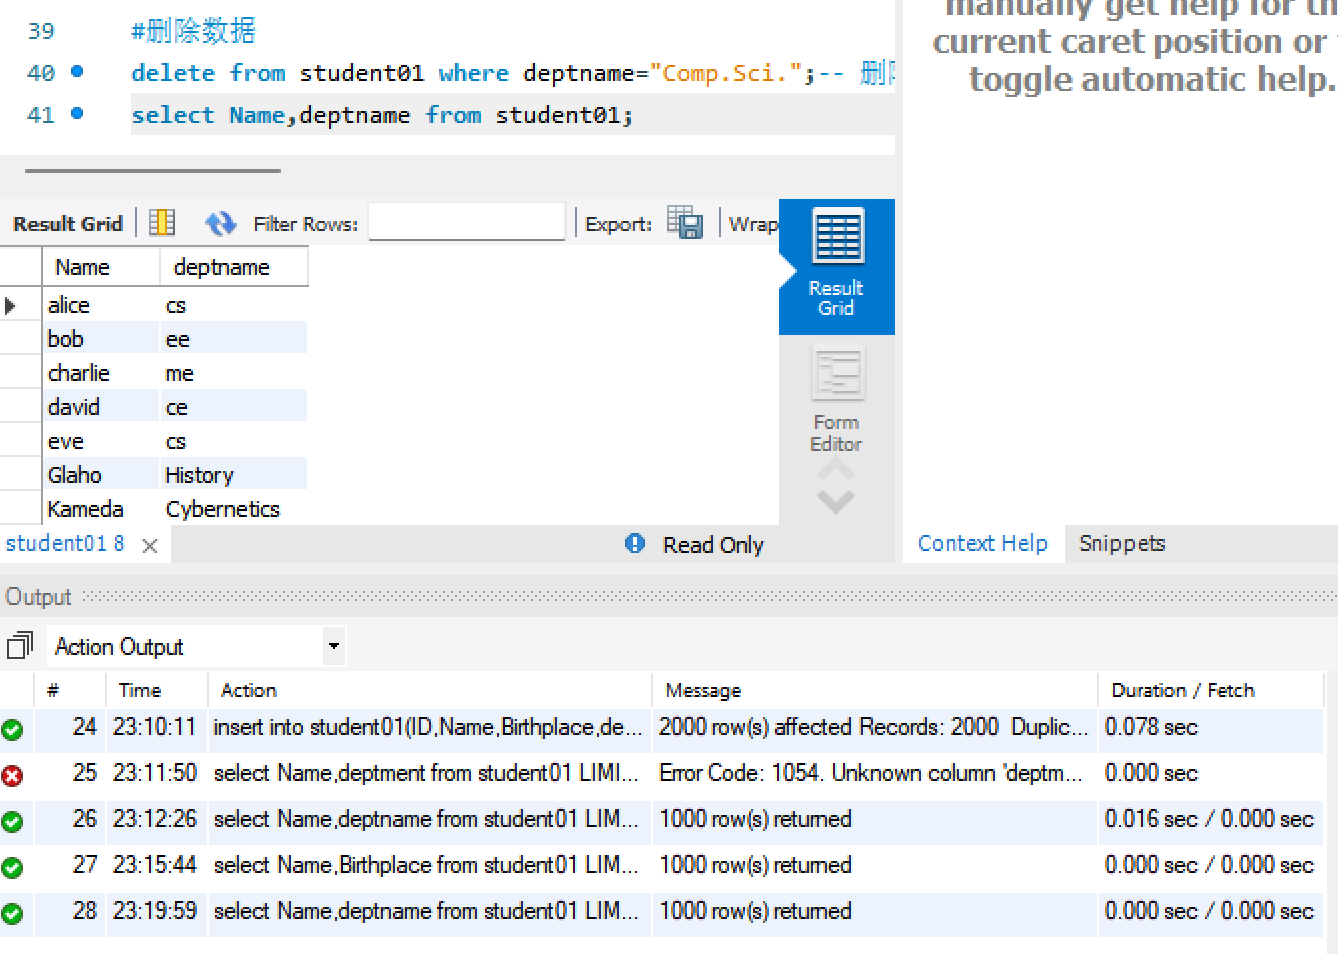
\includegraphics[width=12cm]{figure/image16.png} \\
\footnotesize 图16 简单查询声明相关操作截图4
\end{center}
\vspace{1cm}
\begin{center}
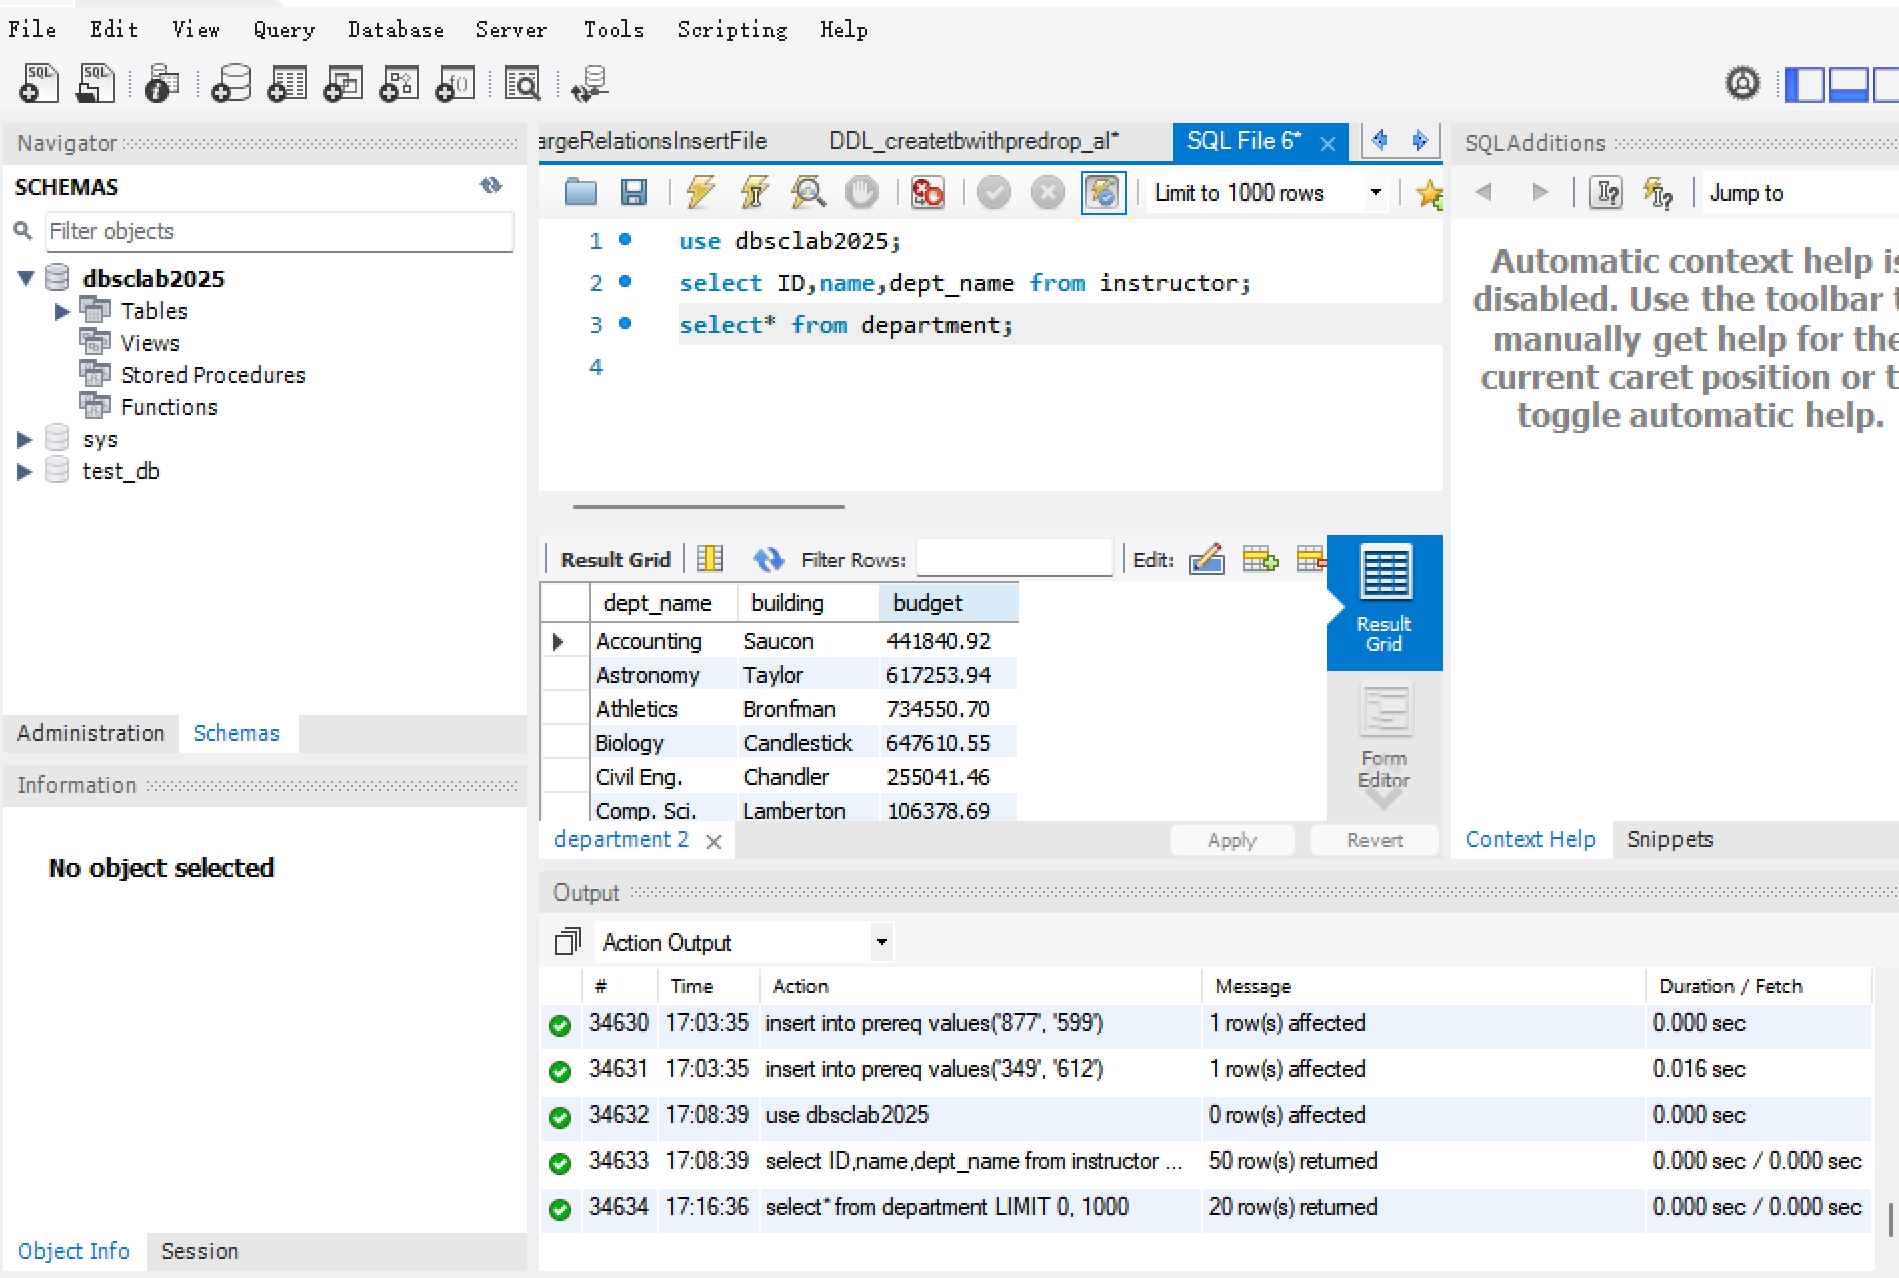
\includegraphics[width=12cm]{figure/image17.png} \\
\footnotesize 图17 简单查询声明相关操作截图5
\end{center}
\vspace{1cm}
\begin{center}
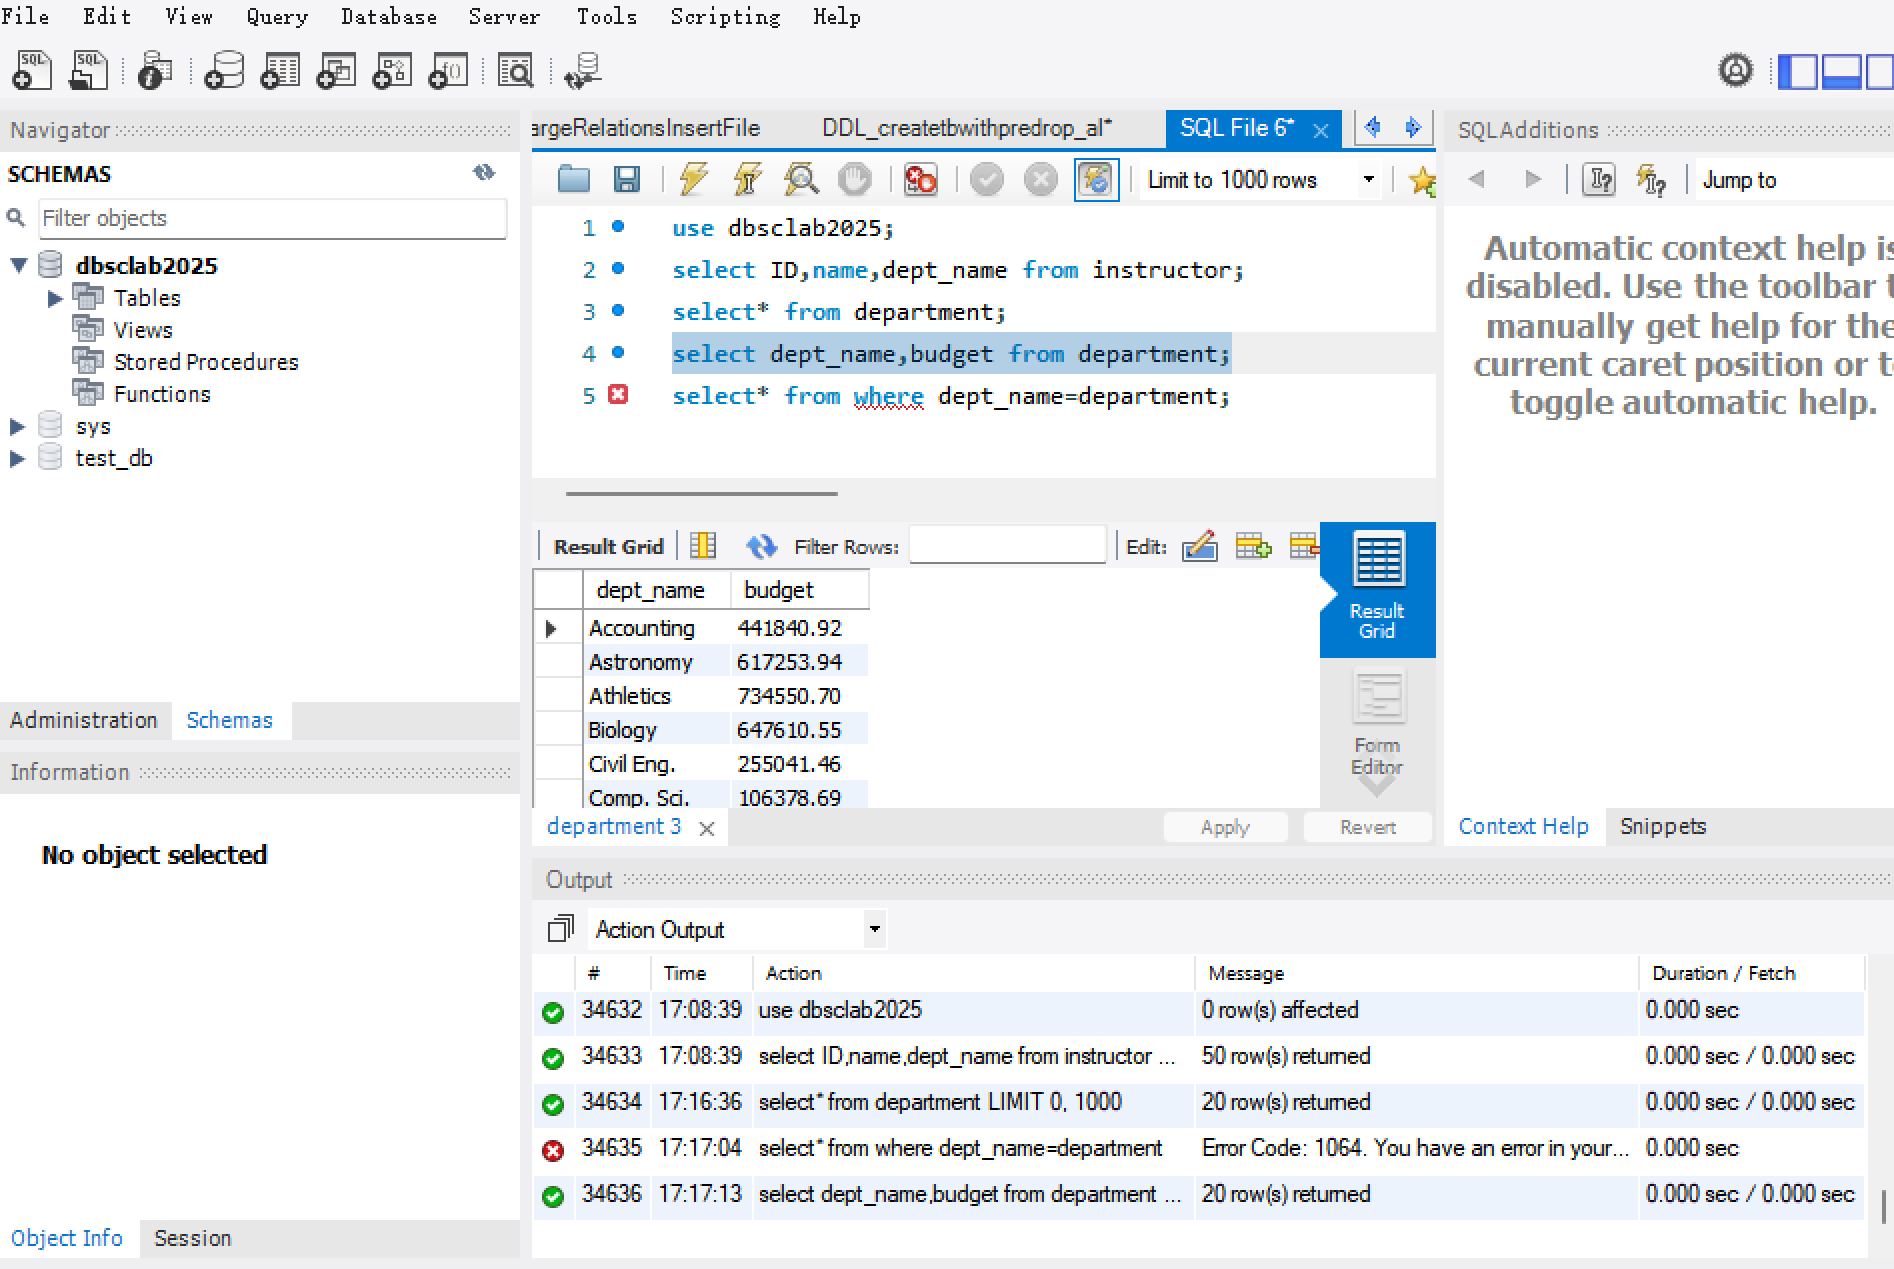
\includegraphics[width=12cm]{figure/image18.png} \\
\footnotesize 图18 简单查询声明相关操作截图6
\end{center}
\vspace{1cm}
\begin{center}
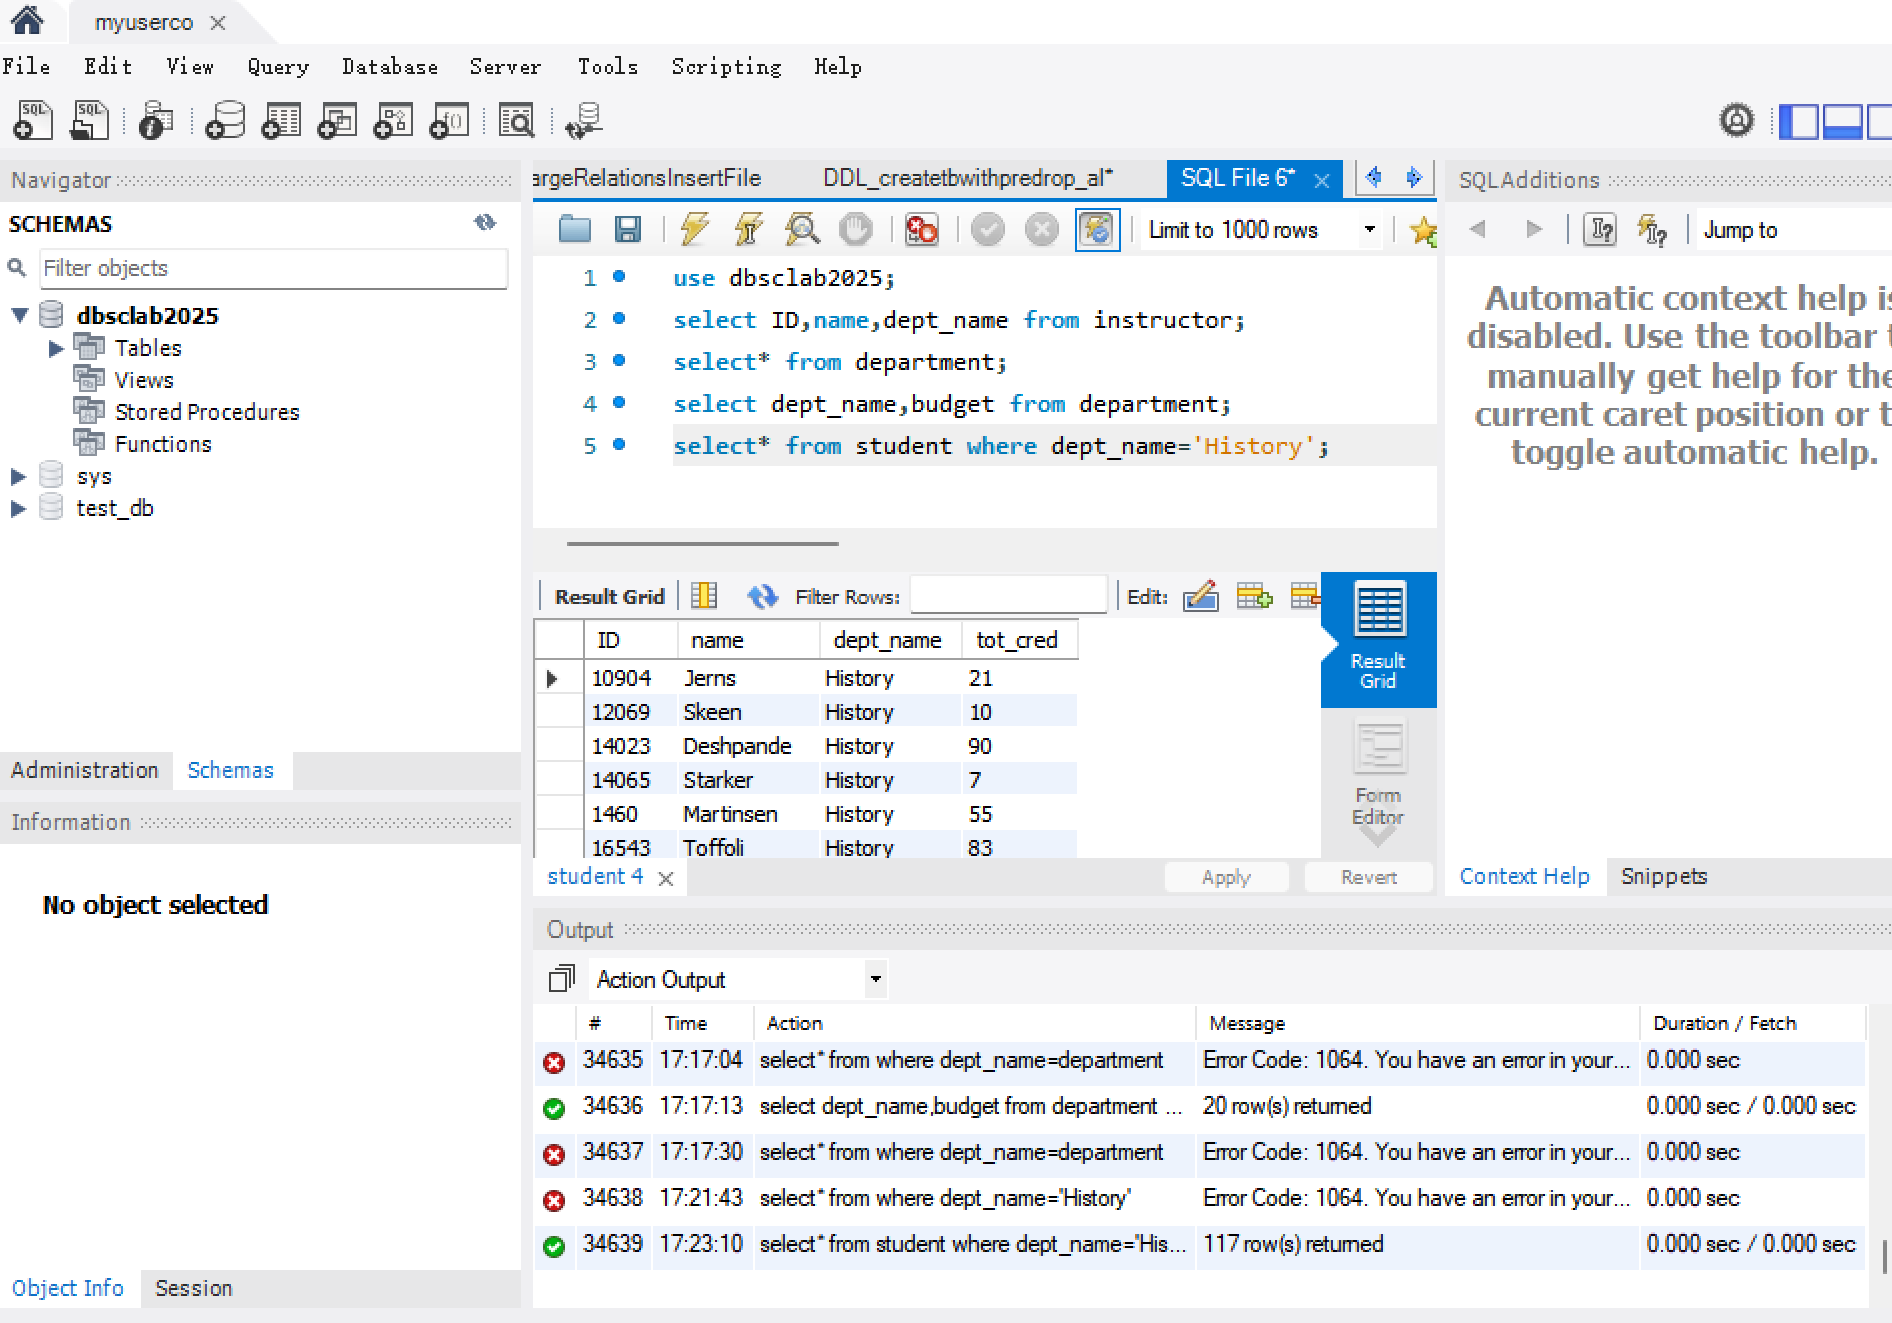
\includegraphics[width=12cm]{figure/image19.png} \\
\footnotesize 图19 简单查询声明相关操作截图7
\end{center}
\vspace{1cm}

\section{QUIZ}
\subsection{方法一：普通CREATE TABLE语句}
\begin{lstlisting}[language=SQL]
CREATE TABLE employees (
    employee_id INT PRIMARY KEY,  -- 员工工号，设为主键
    name VARCHAR(50),  -- 姓名，假设最长50个字符
    age INT,  -- 年龄
    gender ENUM('男', '女'),  -- 性别，使用ENUM类型限定取值
    contact_info VARCHAR(100),  -- 联系方式，假设最长100个字符
    hire_date DATE,  -- 入职时间，使用DATE类型
    salary DECIMAL(10, 2)  -- 工资，总长度10位，小数2位
);
SHOW CREATE TABLE employees;
\end{lstlisting}
\begin{center}
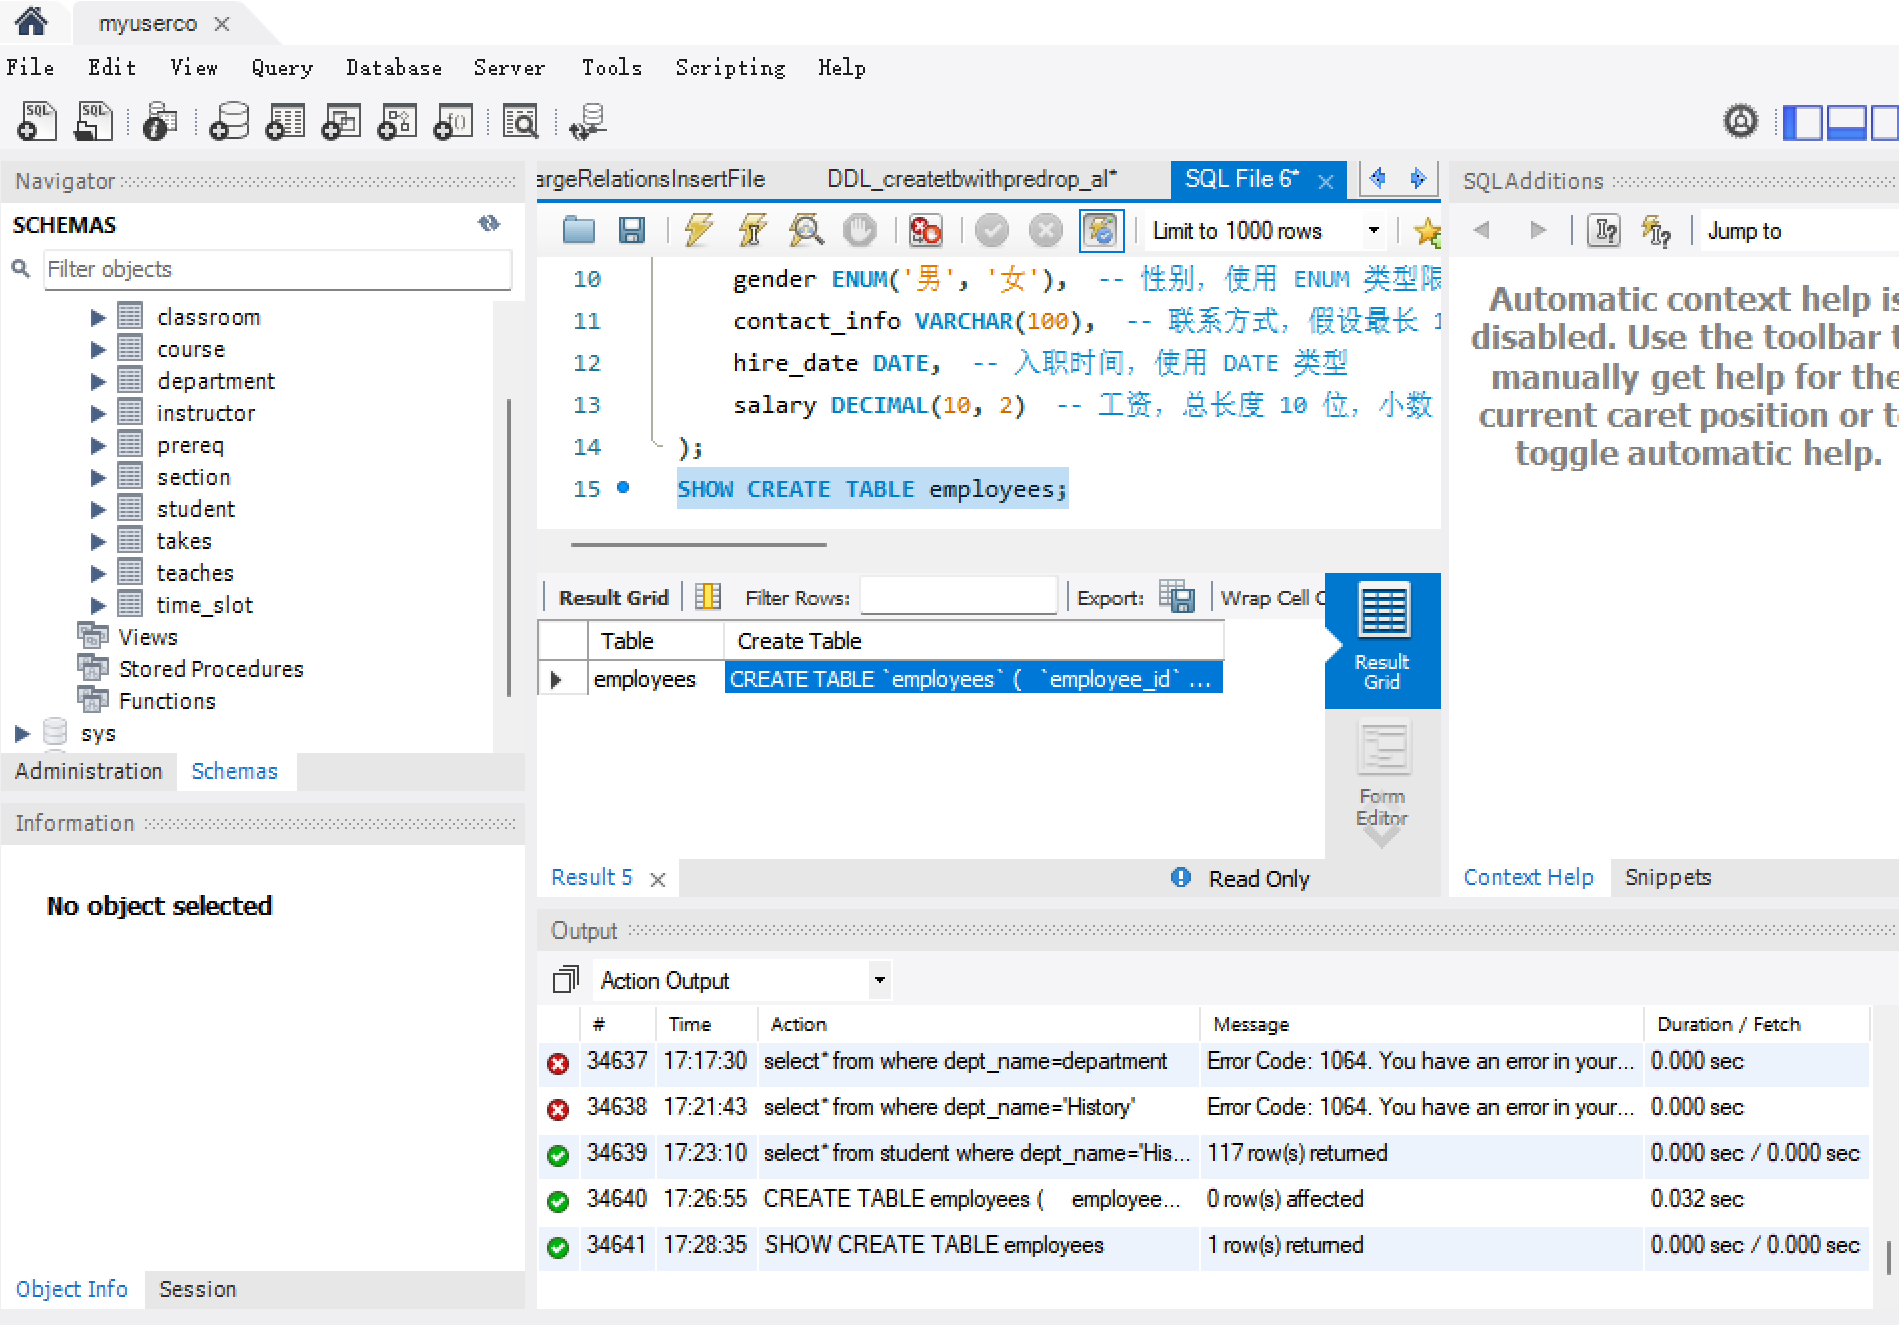
\includegraphics[width=12cm]{figure/image20.png} \\
\footnotesize 图20 普通CREATE TABLE语句操作截图
\end{center}
\vspace{1cm}

\subsection{方法二：通过LIKE复制表结构并修改（先创建一个类似的简单表再修改）}
\begin{lstlisting}[language=SQL]
-- 创建一个简单的基础表
CREATE TABLE temp_employees (
    basic_info VARCHAR(100)
);
-- 通过LIKE复制结构
CREATE TABLE employees1 LIKE temp_employees;
-- 修改表结构，添加所需列
ALTER TABLE employees1
ADD COLUMN employee_id INT PRIMARY KEY,
ADD COLUMN name VARCHAR(50),
ADD COLUMN age INT,
ADD COLUMN gender ENUM('男', '女'),
ADD COLUMN contact_info VARCHAR(100),
ADD COLUMN hire_date DATE,
ADD COLUMN salary DECIMAL(10, 2);
-- 删除临时表
DROP TABLE temp_employees;
SHOW CREATE TABLE employees1;
\end{lstlisting}
\begin{center}
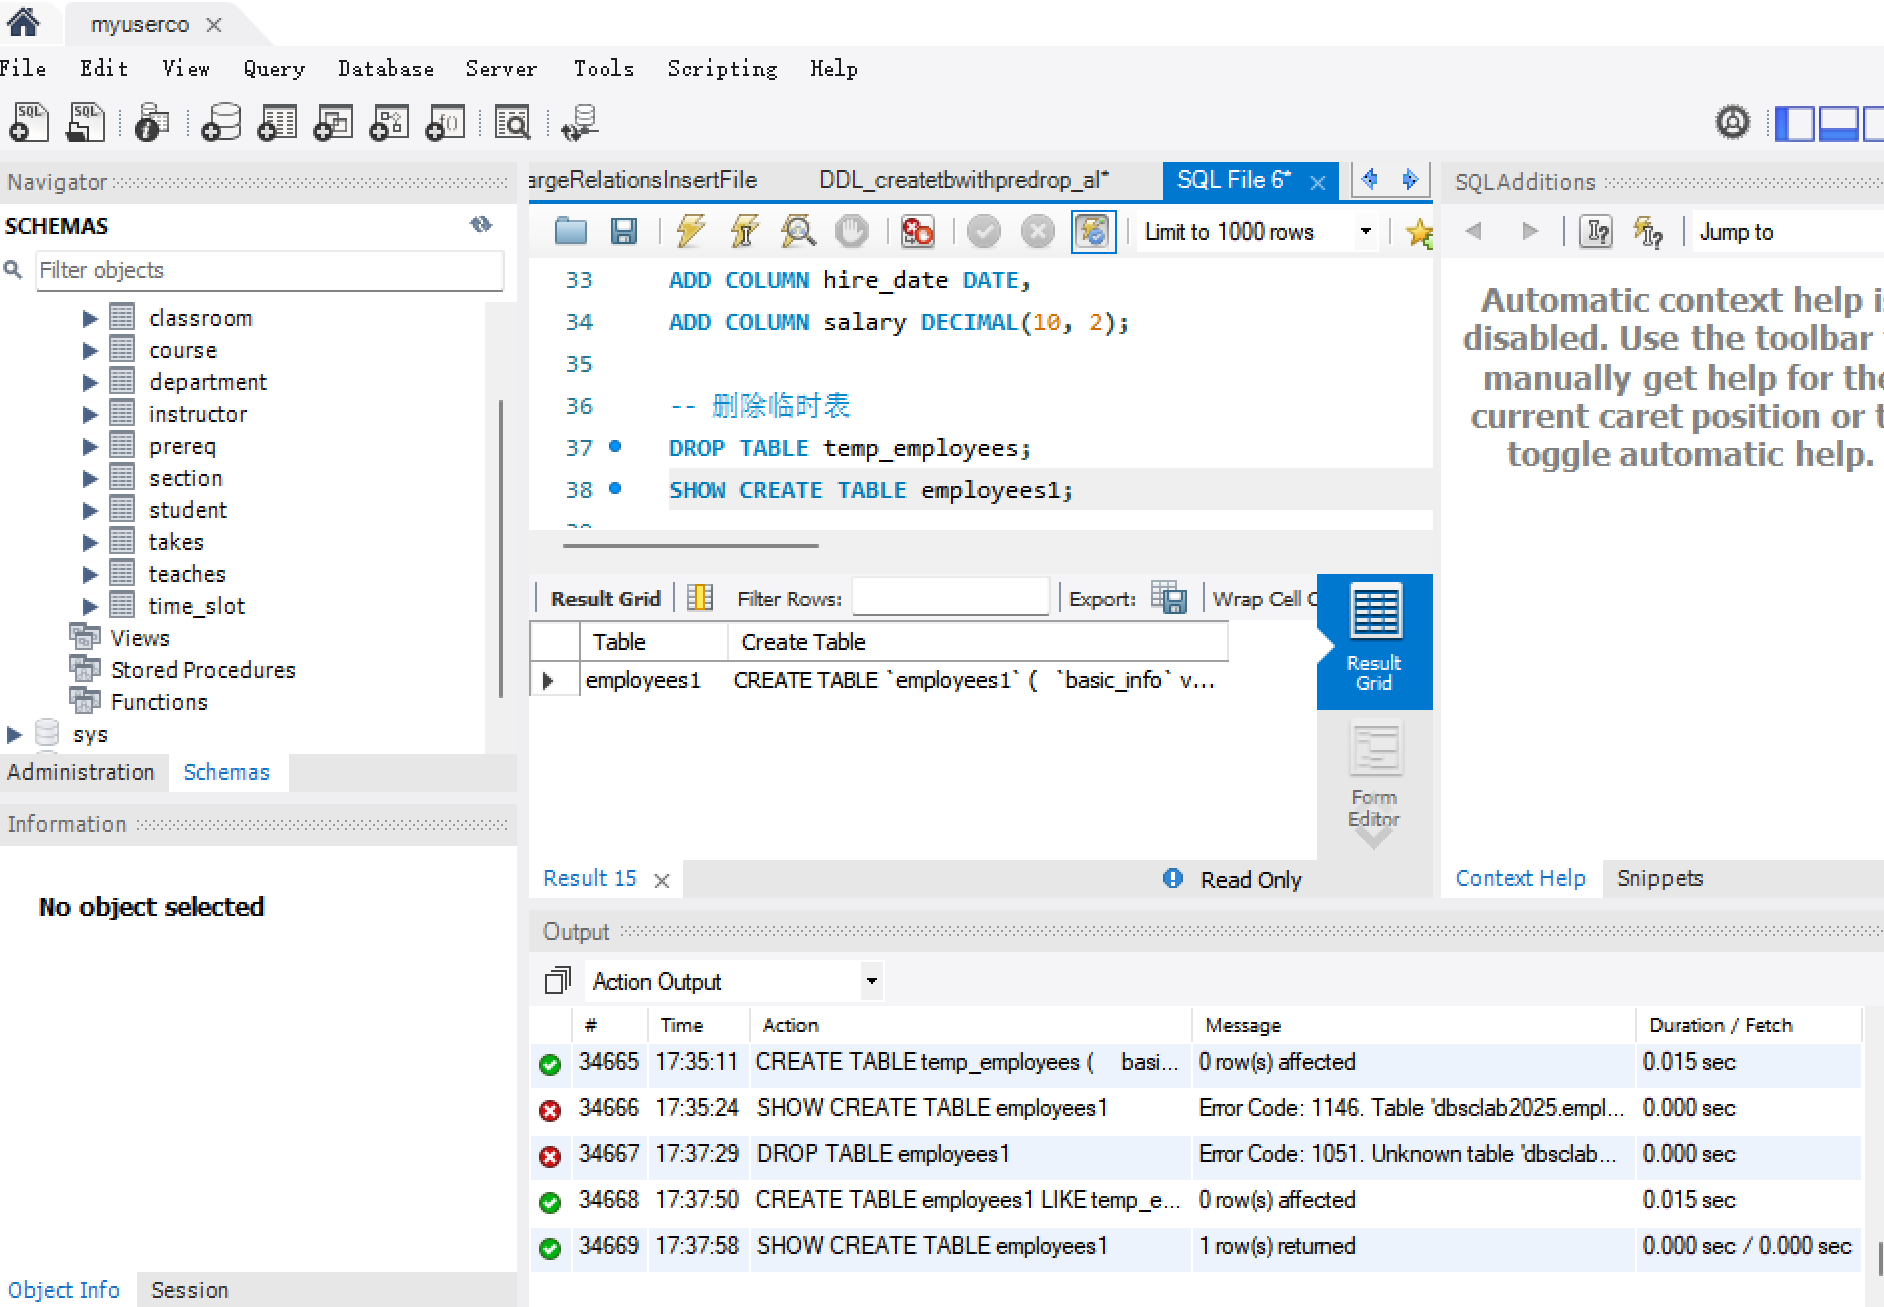
\includegraphics[width=12cm]{figure/image21.png} \\
\footnotesize 图21 通过LIKE复制表结构并修改操作截图
\end{center}
\vspace{1cm}

\chapter{实验结果}
\section{环境配置结果}
Python环境中PyMySQL库安装成功，能正常连接MySQL数据库并获取版本信息，确认数据库版本为8.0.41。

\section{用户管理结果}
新用户`newuser`创建成功并被授予全部权限，可使用该用户连接数据库进行操作。

\section{数据库操作结果}
`dbsclab2025`数据库创建成功，模板数据导入无误，表创建、数据插入和查询操作均按预期执行，复杂查询在修正语法错误后得到正确结果。`employees`和`employees1`表按要求创建，结构和字段符合预期。

\chapter{实验总结}
\section{收获}
1. 熟练掌握了Python与MySQL的连接及数据交互，学会使用PyMySQL库执行数据库操作。
2. 深入理解并掌握了MySQL用户管理和权限分配，能创建用户并灵活设置权限。
3. 精通MySQL数据库和表的创建、数据导入，以及复杂查询语句的编写和调试。

\section{问题与解决}
1. 用户名错误：在配置数据库连接时，因用户名输入错误导致连接失败，通过仔细检查配置信息，修正用户名后成功连接。
2. 查询语法错误：编写复杂查询语句时出现语法错误，如下所示：
\begin{lstlisting}[language=SQL]
select * from where dept_name=department;
\end{lstlisting}
通过查阅SQL语法文档，发现错误并修正，最终得到正确结果。

\section{展望}
本次实验为数据库学习奠定了坚实基础，未来将进一步学习数据库优化、存储过程、索引等高级知识，提升数据库开发和管理能力，以应对更复杂的数据库应用场景。

\end{spacing}
\end{document}